\documentclass[conference]{IEEEtran}
\IEEEoverridecommandlockouts
% The preceding line is only needed to identify funding in the first footnote. If that is unneeded, please comment it out.
\usepackage{multirow,makecell}
\usepackage{cite}
\usepackage{amsmath,amssymb,amsfonts}
\usepackage{algorithmic}
\usepackage{graphicx}
\usepackage{textcomp}
\usepackage{xcolor}
\usepackage{grffile}
\def\BibTeX{{\rm B\kern-.05em{\sc i\kern-.025em b}\kern-.08em
    T\kern-.1667em\lower.7ex\hbox{E}\kern-.125emX}}
\begin{document}
 
\title{(PFF)Political Fact Finder \\
}
\author{\IEEEauthorblockN{Sangwon Kim}
\IEEEauthorblockA{\textit{dept. information system} \\
\textit{Hanyang University}\\
Seoul, Korea  \\
tkddnjs2014@gmail.com}
\and
\IEEEauthorblockN{Kyumin Kim }
\IEEEauthorblockA{\textit{dept. information system} \\
\textit{Hanyang University}\\
Seoul, Korea \\
kkyumin@gmail.com}
\and
\IEEEauthorblockN{Injun Hwang}
\IEEEauthorblockA{\textit{dept. information system} \\
\textit{Hanyang University}\\
Seoul, Korea \\
 sroo2315@gmail.com}
\and
\IEEEauthorblockN{Hyunho Kim}
\IEEEauthorblockA{\textit{dept. information system} \\
\textit{Hanyang University}\\
Seoul, Korea \\
jwalag87@gmail.com}
}
\maketitle
 
\begin{abstract}
The purpose of our service is to help the general public access easily to assembly minutes. The public will be provided not only minutes but also looking up minutes per agenda, participated politicians, his statements, and searching keywords. Through this service, the public can judge politician on real statement, not edited version of media.\linebreak \\
\end{abstract}
 
\begin{IEEEkeywords}
Politician, Speech, Searching system, Assembly Minutes, AI Speaker, Web service  \linebreak \\
\end{IEEEkeywords}
 
  \begin{table}[htbp]
  \renewcommand{\arraystretch}{1.7}
\caption{Role Assignments}
\begin{center}
\begin{tabular}{|p{1.5cm}|p{1.8cm}|p{4.2cm}|}
\hline
\textbf{Roles} & \textbf{{Name}}& \textbf{{Task description and etc.}} \\
\hline
User & NUGU speaker users & The user’s needs are the final goal of the project. They want to make their lives easier and more efficient through the output of the project. They can raise concerns and necessities to the project if their needs don’t meet up to satisfaction. It is the most important their rules in a project.  \\
\hline
Customer & SKT & Customers demand to the project to make satisfied with users. Customers are located between Develop teams and users. The user’s needs through the whole project are really close to the main purpose of their rules because they are closely related to their interests. They want project teams to use NUGU speaker to satisfy users.  \\
\hline
Software \linebreak Developers& Hyunho Kim \linebreak Kyumin Kim& Software developers are main resources of the the project. Their technical stacks and engineering skills create actual product. They demand core function requirements to Development managers which give them up to their developing process. Their final goal is to satisfy users and customers by realizing close to the requirements. \\
\hline
\end{tabular}
\label{tab1}
\end{center}
\end{table}
 
  \begin{table}[htbp]
  \renewcommand{\arraystretch}{1.7}
\begin{center}
\begin{tabular}{|p{1.5cm}|p{1.8cm}|p{4.2cm}|}
\hline
\textbf{Roles} & \textbf{{Name}}& \textbf{{Task description and etc.}} \\
\hline
 
Development \linebreak managers& Sangwon Kim \linebreak Injun Hwang& Development mangers intercommunicate with Customer and Software developer to satisfy with whole stakeholders. They schedule timelines to stick to the project before deadline. They build overall developing design process. So they should figure out what they are confronted by, such as threats and variables, plan projects and direct business matters that Software developers can’t handle with. They support Software developers to focus on developing processes. \\
\hline
\end{tabular}
\label{tab1}
\end{center}
\end{table}
 
\vspace{17mm}


\section{Introduction}
In Korea, there’s a fashioned sentence “The general publics are dog and pig”. This sentence was just a script of Korean movie, “Insiders”, but it gives sympathies to many citizens. Our team started to think about why this sentence is caught in the minds of the people.
 
The articles of Korean presses tend to be written on suggestive, prejudiced by inclination of that press rather than political facts, while editing politician’s opinions or moves. Also, the presses tend to report only in just portion of facts, only in favor of certain political orientations. Consequently the public can’t decide whether that article is neutral or biased on amicable organizations. So they tend to be instigated by that biased report quite often unknowing the facts. In fact, when looking at Naver(the largest portal site of Korea)’s political news article, a lot of people are instigated, unilaterally and aggressively commenting on the contents due to stimulating titles or contents that mixed with specific utterances and reporters' opinions. So Naver often hides highest recommended comments in such articles.

Furthermore, by the research of "Statista, Reuters Institute Disital News Report 2018", Worldwide fake News are seriously produced, and Korea ranked 5th. Also, by the research of "Tomorrow university 20th laboratory" reported 43.3 percent of people are encountered fake news more than once a week. To deal with this situation, Government and Assembly should check this situation and make suitable actions.
 
It means there is a lack of fact information that politics can’t judge politician objectively. Current articles are processed based on reporter’s political orientation, so people are more and more complicated, and can’t make decide based on their criteria. To escape on this situation, some people make an effort to access on assembly site to judge that certain politician’s utterances and their political orientation. But, finding information only on facts is not just easy. It brings about three problems below.
 
First, the most objective way to determine what a politician has spoken is to hear and judge pure speech of politician, not someone else’s refined words. Usually, the politician speaks something that is full of political beliefs in the political meeting. It would be a fact information that politic can determine about the politician. The public fact data of the politician in the assembly site are just only on election records, award records, criminal facts, etc. These simple examples don’t provide inclination of the politician. Hence, our team got conviction that the real opinion of politician is in the congressional records. Therefore, our team will develop a service that can verify what politician has spoken by serving  assembly minutes easily.
 
Second, the way to find congressional records is too complex. Congressional records in the assembly are typed by stenographer, and opened to the public through National Assembly Minutes. Public should link in National Assembly Minutes System and download pdf files to find remarks. Many citizens don’t interested in politics because it doesn’t give any monetary benefits or it doesn’t give fun to them. To turn their minds, minimized way to get information of politicians is needed. The National Assembly Minutes that doesn’t provide convenience to the citizen is just a nominal system. So our team decide to give information about Assembly minutes to citizen easily through web page. Also, we would like to use AI speaker to fulfill desires of various people.
 
Furthermore, the current minutes is not classified of its contents and politicians. The file name of minutes just designates on conference date and order. If the user wants to find specific agenda, they need to search it manually by scrolling the pdf files. So our team decide to give solution of this problem. We are going to parse all of the minutes and after classify the politician’s agenda and speech in the minutes. This service will provide an useful function that search specific agenda and politician to users. It will be applied to AI speaker to make our service more useful.
 
The AI speaker(Smart speaker) is a kind of wireless speaker, which is activated by more than one impressive words(hot words). Voice-Command-Device wh ch embed The Virtual Assistant carries out co-interactive functions and hands-free commands.
 
The biggest difference between AI Speaker and typical Speaker is that the AI speaker recognizes “Speech Recognition” to perform specific commands like listening to music, setting alarm and timer, searching information like News, weather, etc. The main input and output unit of Speech-Recognition device is built-in Microphone and Speaker. The AI speaker is consisted of such like these simple units, so it is efficient to send and receive information than any other smartphone, smart TV.
 
Specifically, The NUGU speaker is the first Korean-made AI speaker made by SKT in 2016. Over the last two years, The NUGU speaker so far developed a lot so typical functions such as mentioned above are already applied. So our team had to decide to make service that speaker doesn’t provide and groundbreaking service
 
Third, There is no current services that gather personalized inclined politician or his related field. By lacking of information of politicians, just some specific politicians are reminded to citizens. Though, even if the politician is not popular, some people’s area of interest can be similar to him. Maybe they want to subscribe regularly of that politician. When they want to find information of him, but they will find out that there are only refined, edited version of his mentions. So, based on whole minutes of specific politician’s participated, we will make a interested area or keyword extraction service through big data analysis for our big future plan. This will be a good method to listen on politician who is similar to user’s interested area by setting up user’s keyword of interested area and scrapping of his activation.
 
In conclusion, we want to make a  personalized subscribe system of interested politician so the politic can determine of the politician based on objective facts. For this, our team will make service that meet four functions. first, recognizing specific politician’s statements by looking up assembly minutes. second, printing the words through web service and AI speaker. third, the function that finding agenda or politician easily. fourth, a method of searching system that user can input his interested words and mentions in the article and the system print outputs the most realated log. Through this service, It is anticipated that the public’s independence and judgement will be improved.
 
 \vspace{90mm}

\section{Requirements}
\subsection{Public}

The public can be provided with  not only providing information on the minutes of the assembly but also detailed functions of the minutes. It consists of Log-in page and Main page as big category. They can be provided various useful functions like Looking up function about meeting contents per agenda, participating specific politicians, and their real speech in that agenda.Subscribing interesting politicians and searching keywords system are also provided. \\ 
 
\begin{enumerate}
    \item \textit {Log-in Page:} 
In the log-in page, the user can saves specific politicians or interested keywords individually. subscribed politician, interested keywords are saved in back-end server. through this, the user can uses subscribe or registering functions.\\
    \begin{enumerate}
        \item \textit {Sign-up:}  Log-in page is a first page that users can see when they enter to our website. If username and password are match to our database, user can log in our web page to use our personalized system.\\
        \item \textit {ID/PW search:} When the user forgets their id or password, this function can find their ID or password after  certificating process.\\
    \end{enumerate}
    
    \item \textit {Main Page:}  The main page is a key feature of this service. Users can search for detailed information about minutes. To concrete this, the following functions are implemented. \\
    
      \begin{enumerate}
    \item \textit{Basic components residing whole web-site:} It consists of website's basic components like Navigation bar that contains several link on whole web page and footer that contains subordinate information. Also, our web service's overall color concept is based on black-navy color. \\
            \begin{enumerate}
    \item \textit{Navigation bar:} it contains several components of the application and user can can navigate to the selected page by selecting the list. \\
    
    \item \textit{Footer:} It resides on our whole web page in upper side to make our user see our team information easily.
    \\
        \end{enumerate}
            \end{enumerate}
    \begin{enumerate}
        \item \textit {Looking up function about meeting contents per agenda:} Users can view agendas entering by organized meeting contents following  three pages. Each pages intercommunicate to user to surf easily our web service.\\
        \begin{enumerate}
            \item \textit {Looking up list of assembly minutes:} Users can view list of assembly minutes. Each minutes are classified by kinds of that minutes. If user click a minutes, he go through the next page.\\
            \item \textit {Looking up list of agendas per specific assembly minutes:} Users can view list of agendas held on specific minutes. If user click a agenda, he go through the next page.\\
            \item \textit {Looking up dialogue of specific agenda:} Users can view politician's dialogue that held on specific agenda. The dialogue looks like each politician talks each other. \\
            
        \end{enumerate}
      
        
        \item \textit {Looking up function about politicians' speech according to agenda:} User can view politician's personal information page. This page consists of what meeting, what agenda the politician participated in and his or her utterances in that agenda.  \\
        
        \item \textit {Looking up function about subscribing politicians:} Users can view specific politicians that the user was subscribed. User can customize by following politicians.\\
        
        \item \textit {Searching real speech of the politician function:} Users can search interesting keywords or quotations from articles, news, etc. Search Engine will find real speech of the politicians and agendas. \\
        
        \item \textit {Looking up function about politician list:} User can view politician list. User can view current members of assembly along with what political party they are belonged to.\\
        
        \item \textit {Registering of interested political keyword:} User can input his interested keywords to his profile. Also, users can be recommended about politicians by entering interested keywords. \\
        
        \item \textit {Subscribing function about interesting politicians:} Users can subscribe about interesting politicians. This function can be spotted on anywhere on our web service for easy and convenient use of service.\\
        \end{enumerate}
    \end{enumerate}

    \begin{enumerate}
        \item \textit{Nugu service:} User can use our service through Nugu speaker. They can input specific utterance and the Nugu speaker answers back to the users. At this side, three functions should be implemented.\\
        
        \begin{enumerate}
        \item \textit{Searching information of the politicians function:} This function can search politician’s participated agendas. If the user utter curious politician, Nugu speaker send back most recent participated agenda of the politician.\\
        
        \item \textit{Looking up real speech of the politician in that agenda:} User can look up real speech of the politician. Nugu speaker speak out specific politician’s most recent utterance.\\
        
        \item \textit{Changing real speech of the politician in that agenda:} User can request Nugu speaker to play back or forward speech of the politician. Nugu speaker speak out back and forward speech of current playing.\\
        
        \item \textit {Subscribing function about interesting politicians:} Users can subscribe to interesting politicians by ordering to Nugu.\\
        
        \item \textit {Deleting subscribed politicians function:} Users can delete subscribed politicians what he registered by ordering to Nugu. \\
           \end{enumerate}
    \end{enumerate}
    
    
    
    
    
    \vspace{300mm}

\section{Related Works}
We have researched for some softwares that are doing similar works or having similar services to ours. There are some tools that are providing similar service in the side of political things, with  different logics and platform . By doing this research, we found out that software about politics is widely used in various kinds of fields and it has a lot of potential powers. 
 
\subsection{g0v}
  \begin{figure}[htbp]
    \centerline{
\includegraphics[width=89mm, scale=0.5]{fig/111.png}}
    \caption{g0v}
    \label{fig}
    \end{figure}
The g0v is an open source, open government collaboration started by Chia-liang Kao, ipa, kirby and others in late 2012 in Taiwan. Originally driven by a bimonthly hackathon, the community has expanded to include different professional and non-information technology background members. a "forked" version of that agency with contributions by civic hackers. Continuing this inspiration from the software development world, the forked content can then be "merged" back into the government agency's website. g0v is a community that promotes the transparency of government information and is committed to developing information platforms and tools for citizens to participate in society. As of the beginning of 2014, there have been contributors across three continents, and the results have been released in a free software model that embraces knowledge sharing.
\\
\\
 
\subsection{Gov track}
  \begin{figure}[htbp]
    \centerline{
\includegraphics[width=89mm, scale=0.5]{fig/gov_track.jpg}}
    \caption{Gov track}
    \label{fig}
    \end{figure}
    
GovTrack.us is a website developed by then-student Joshua Tauberer. It is based in Washington, D.C., and was launched as a hobby. It enables its users to track the bills and members of the United States Congress. Users can add trackers to certain bills, thereby narrowing the scope of the information they receive. The website collects data on members of Congress, allowing users to check members' voting records and attendance relative to their peers. It propagates the ideology of increasing transparency in the government and building better communication between the general public and the government.
 \vspace{20mm}

 
\subsection{sunlight foundation}
  \begin{figure}[htbp]
    \centerline{
\includegraphics[width=89mm, scale=0.5]{fig/sunlight_foundation.png}}
    \caption{sunlight foundation}
    \label{fig}
    \end{figure}
The Sunlight Foundation is an American 501 nonpartisan, nonprofit organization that advocates for open government. The organization was founded in April 2006 with the goal of increasing transparency and accountability in the United States Congress, the executive branch, and in state and local governments. The foundation's primary focus is the role of money in politics. The organization seeks to increase campaign finance regulations and disclosure requirements.The Sunlight Foundation advocates for more regulation and limitations regarding campaign finance. The organization opposed the ruling in Citizens United v. FEC, calling it "disastrous.". The organization supported the DISCLOSE Act, a congressional bill that would have enacted stricter campaign finance regulations by requiring increased disclosure of political spending in federal elections. The Sunlight Foundation believes that Congress should mandate real-time online disclosure of political contributions. It opposes dark money, or funds given to nonprofit organizations that are not required to disclose their donors.
\\
 \vspace{25mm}

\subsection{Brigade media}
  \begin{figure}[htbp]
    \centerline{
\includegraphics[width=89mm, scale=0.5]{fig/brigade_media.jpg}}
    \caption{Brigade media}
    \label{fig}
    \end{figure}
Brigade Media, also known as Brigade, is a civic technology platform that was formed on June 4, 2014, and founded by James Windon, Jason Putorti, John Thrall, Matt Mahan, and Miche Capone. The platform is intended to serve as a way for users to connect with others who share the same or similar views and voice their opinions, create debates, or organize petitions. This process is intended to make the users' concerns more visible to and influential towards United States' policymakers. One mission of Brigade Media is to act as a foreground for its users to connect and organize so that they can voice their opinions on our nation's issues. Another more general goal is to increase voter participation. Brigade interacts with American voters by linking its users to the same held concerns. The opinions of elected officials on those concerns will be provided and metrics about the candidate most similar in concerns and degree of concern will be available. This data should be useful for both candidates and voters, in that voters can voice their grievances and candidates must respond accordingly.
 \\
 
  \vspace{90mm}

\section{Development Environment}
\subsection{Choice of development platform}
\begin{enumerate}
  \item 
  \textit{Used platform and why}
    
We will going to use Linux OS platform, specifically Ubuntu ver 16.04 LTS.  (Ubuntu is free, completely customizable, resource-friendly than Windows platform.) Furthermore, Linux command line is the biggest reason to use this platform. Its Bash(Shell) with a various command makes our development process easy.
In addition, our team going to use Amazon Web Service(AWS) to upload our service to cloud server. Amazon Elastic Compute Cloud (EC2) is a leading infrastructure cloud service that offers scalable compute capacity in the cloud. It allows clients to rent powerful virtual computers and run their own applications. To use this, we have to boot an Amazon Machine Image(AMI). AMI Ubuntu ver 16.04 LTS is provided by the AWS in free tier, so we decide to use. Continuity with local OS version with server OS version helps to develop without incompatibility that occured due to OS differences.
\\
  
   \item \textit{Used Programming Language and why}
       \begin{enumerate}
        \item \textit{Python 3.7}
\\The Python Package Index(PyPI) contains numerous third-party modules that make Python capable of interacting with most of the other languages and platforms. Python provides a large standard library which includes areas like internet protocols, string operations, web services tools and operating system interfaces. Many high use programming tasks have already been scripted into the standard library which reduces length of code to be written significantly.\\
 
        \item \textit{Java 1.8}
 \\When use spring, the Java language framework, it provides comprehensive infrastructure support for developing Java based applications. Spring also enables the developer to create high performing, reusable, easily testable and loose coupling enterprise Java application. So to speak, Spring provides an abstraction layer on existing technologies like servlets, jsps, jdbc, jndi, rmi, jms and Java mail etc., to simplify the development process. Spring also provides a light-weight container which can be activated without using web server or application server.\\
    
            \item \textit{Javascript}
 \\Vue.js, a Javascript framework with various optional tools for building user interfaces, is  widely used across the world for web development. One of the greatest advantages of Vue.js is its small size. The size of this framework is 18–21KB and it takes not much time to download. Also, it is quite easy to understand. In simple web structure like our project software, Vue.js can be easily added. The documentation with Vue.js is so comprehensive so we can develop our service quickly and concretely.\\
    
            \item \textit{HTML5}
 \\ HTML is one of the best option to develop the webpage or website for the small or growing business that does not want to invest more in purchasing software or its license and does not require any advanced programming for their websites. HTML provides an easy way to optimize the website in HTML according to browsers to the web developers. HTML can be easily integrated with multiple languages and does not create any issues in it. The most important thing is HTML is used in frontend development for over so many years before we have no other languages available in the market for web development.\\
 
            \item \textit{CSS}
 \\ CSS allows for more control over the presentation of our web pages. The Style Sheets specification works by allowing to specify rules that say how the content of elements within our document should appear. One of its key benefits is the way it allows the separation of document content. Converting from an HTML page to a CSS design page may be a bit difficult and time consuming task. So, we decide to use CSS.\\
    \end{enumerate}
    
     \vspace{97mm}

  \item \textit{Cost estimation (Software): } 
  \begin{table}[htbp]
  \renewcommand{\arraystretch}{1.5}
\caption{Cost estimation}
\begin{center}
\begin{tabular}{|p{3cm}|p{3.7cm}|p{0.5cm}|}
\hline
\textbf{Category       } & \textbf{Name and Version   } &\textbf{Cost} \\
\hline
Operating System &Ubuntu  16.04 LTS&0 \\
\hline
VMware & VirtualBox 5.2.20&0 \\
\hline
Search Engine & Elasticsearch 5.7 &0 \\
\hline
\multirow{2}{*}{Text editor} & Sublime text 3 &0 \\
& Visual Studio Code 1.39 &0  \\
\hline
IDE & Eclipse 20188-12 &0 \\
\hline
Development Kit & JDK 1.8 &0 \\
\hline
\multirow{2}{*}{Version control} & Git &0 \\
& Github &0 \\
\hline
Server & AWS EC2(free tier) &0\\
\hline
\multirow{2}{*}{Documentation}&  Latex &0\\
& Google Docs &0\\
\hline
\multirow{2}{*}{Communication} & Slack &0\\
& KakaoTalk &0\\
\hline
Design & Balsamiq&0\\
\hline
\end{tabular}
\label{tab1}
\end{center}
\end{table}
\end{enumerate}
 
\subsection{Software in use}
\begin{enumerate} 
  \item \textit{Git } 
    \begin{figure}[htbp]
    \centerline{
\includegraphics[width=89mm, scale=0.5]{fig/git.png}}
    \caption{Git}
    \label{fig}
    \end{figure}
  \\The Git is a distributed version-control tool. So to speak, Git can review previous version easily, when it comes to complicated codes. Many users can share their entire codes dividing their part, even if they are developing same module. Even if the network doesn’t work, the user can version control their codes until network works.\\
  
    \vspace{50mm}

   \item \textit{Github} 
       \begin{figure}[htbp]
    \centerline{
\includegraphics[width=89mm, scale=0.5]{fig/github.png}}
    \caption{Github}
    \label{fig}
    \end{figure}
   \\The Github is a web hosting service which uses Git. Github provides graphical user interface(GUI) Web UI, In contrast to Git(CLI). Github projects can be operated through Git CLI interface. In addition, Open repository of Github can be visited not only registered users but also non-registered users. So, when the another user wants to fork other person’s repository, they can fork theirs. One of a function of Github is pull requests, that is, when the other users want to push modified codes, the original author can review their codes and can confirm to change his code. \\
   \item \textit{AWS }
          \begin{figure}[htbp]
    \centerline{
\includegraphics[width=89mm, scale=0.5]{fig/aws.png}}
    \caption{AWS}
    \label{fig}
    \end{figure}
   \\Amazon Web services(AWS) is a subsidiary of Amazon that provides on-demand cloud computing platforms to individuals, companies, and governments as they pays. AWS provides various infrastructures and gathered service that every physical computing resources such as Web and mobile applications, big data projects, social game can executed through cloud system. The AWS technology is implemented at server farms throughout the world. Subscribers can obtain large scale computing capacity more quickly and cheaply. than building an actual physical server farm. It is known as most safe and trustable cloud service in the world. It also has easy and fast expandability. \\
   \item \textit{Sublime text } 
             \begin{figure}[htbp]
    \centerline{
\includegraphics[width=60mm, scale=0.5]{fig/sublime.png}}
    \caption{Sublime text}
    \label{fig}
    \end{figure}
   \\Sublime Text is a proprietary cross-platform source code editor with a Python application programming interface (API). It natively supports many programming languages and markup languages, and functions can be added by users with plugins, typically community-built and maintained under free-software licenses.\\
   \item \textit{Slack }
                \begin{figure}[htbp]
    \centerline{
\includegraphics[width=60mm, scale=0.5]{fig/slack.png}}
    \caption{Slack}
    \label{fig}
    \end{figure}
   \\Slack is a cloud-based proprietary instant messaging platform developed by Slack Technologies. Slack offers many Internet Relay Chat(IRC) features, including persistent chat rooms(channels) that is organized by topic, private groups, and direct messaging. By using Slack, users can find previously uploaded files easily in the messenger. Users also can communicate on its each files. Users can communicate on each topics, and can comment on individual messages.\\
   \item \textit{Latex }
                   \begin{figure}[htbp]
    \centerline{
\includegraphics[width=89mm, scale=0.5]{fig/latex.png}}
    \caption{Latex}
    \label{fig}
    \end{figure}
   \\Latex is a document preparation system. When writing, the writer uses plain text as opposed to the formatted text like word processors like Word. The writer uses markup tagging conventions to define the general structure of a document, to stylise text throughout a document, and to add citations and cross-references. Latex is widely used in academia, and it can be used as a standalone document preparation system, or as an intermediate format. LaTeX is intended to provide a high-level, descriptive markup language that accesses the power of TeX in an easier way for writers.\\
   \item \textit{Google Docs }
                   \begin{figure}[htbp]
    \centerline{
\includegraphics[width=89mm, scale=0.5]{fig/google.jpg}}
    \caption{Google Docs}
    \label{fig}
    \end{figure}
   \\Google Docs is a word processor included as part of a free, web-based software office suite offered by Google within its Google Drive service. The application allows users to create and edit files online while collaborating with other users in real-time. Edits are tracked by user with a revision history presenting changes. An editor's position is highlighted with an editor-specific color and cursor. A permissions system regulates what users can do.\\

  \vspace{30mm}

   \item \textit{Balsamiq }
                   \begin{figure}[htbp]
    \centerline{
\includegraphics[width=60mm, scale=0.5]{fig/balsamiq.png}}
    \caption{Balsamiq }
    \label{fig}
    \end{figure}
   \\Balsamiq Wireframes is a graphical user interface that is website wireframe builder application. It allows the designer to arrange pre-build widgets using a drag-and-drop WYSIWYG editor. Balsamiq Wireframes is a rapid low-fidelity UI wireframing tool that reproduces the experience of sketching on a notepad or whiteboard, but using a computer. It really forces to focus on structure and content, avoiding lengthy discussions about colors and details that should come later in the process.\\
    \item \textit{virtualbox }
                    \begin{figure}[htbp]
    \centerline{
\includegraphics[width=89mm, scale=0.5]{fig/virtual_box.jpg}}
    \caption{virtualbox}
    \label{fig}
    \end{figure}
   \\Oracle VM VirtualBox is a free and open source hosted hypervisor for x86 virtualization. it can be installed on various operating system like Windows, MaxOs, Linux, etc. It supports the creation and management of guest virtual machines that runs Windows, Linux, limited macOS. User can load multiple guest OSs under single host operating system. Each guest OS can be started, paused, and stopped independently within its own virtual machine.\\
   \item \textit{JDK }
                   \begin{figure}[htbp]
    \centerline{
\includegraphics[width=89mm, scale=0.5]{fig/jdk.png}}
    \caption{JDK}
    \label{fig}
    \end{figure}
   \\Java Development Kit is an implementation of various platform released by Oracle Corporation aimed at Java developers on Linux, macOS or Windows. It includes a private JVM and a few other resources to finish the development of a Java Application.  The JDK comes with a complete Java Runtime Environment(JRE) that composed with  Java Virtual Machine(JVM) along with all of the class libraries. Also, it includes Java Compilers, Debuggers, JavaDoc that needed to develop Java software.\\
      \item \textit{Eclipse}
                      \begin{figure}[htbp]
    \centerline{
\includegraphics[width=89mm, scale=0.5]{fig/eclipse.png}}
    \caption{Eclipse}
    \label{fig}
    \end{figure}
   \\Eclipse is an integrated development environment used in computer programming, and it was most widely used Java IDE in one website’s poll in 2014.  It contains a base workspace and an extensible plug-in system for customizing the environment. Eclipse is written mostly in Java and its primary use is for developing Java applications. Development environments include the Eclipse Java development tools (JDT) for Java.. Eclipse supports development for Tomcat, GlassFish and many other servers and is often capable of installing the required server (for development) directly from the IDE. It supports remote debugging, allowing a user to watch variables and step through the code of an application that is running on the attached server.\\
   
   \vspace{30mm}

      \item \textit{Visual Studio Code }
                      \begin{figure}[htbp]
    \centerline{
\includegraphics[width=89mm, scale=0.5]{fig/vscode.png}}
    \caption{Visual Studio Code}
    \label{fig}
    \end{figure}
   \\Visual Studio Code is a source-code editor developed by Microsoft for Windows, Linux and macOS. It includes support for debugging, embedded Git control and GitHub, syntax highlighting, intelligent code completion, snippets, and code refactoring. It is highly customizable, allowing users to change the theme, keyboard shortcuts, preferences, and install extensions that add additional functionality. Visual Studio Code is a source code editor that can be used with a variety of programming languages. Instead of a project system it allows users to open one or more directories, which can then be saved in workspaces for future reuse.\\
   
      \vspace{20mm}

      \item \textit{Elasticsearch }
                      \begin{figure}[htbp]
    \centerline{
\includegraphics[width=89mm, scale=0.5]{fig/elasticsearch.png}}
    \caption{Elasticsearch}
    \label{fig}
    \end{figure}
   \\Elasticsearch is a search engine based on the Lucene library. It provides a distributed, multitenant-capable full-text search engine with an HTTP web interface and schema-free JSON documents. Elasticsearch is developed in Java. Following an open-core business model, parts of the software are licensed under various open-source licenses. Elasticsearch can be used to search all kinds of documents. It provides scalable search, has near real-time search, and supports multitenancy.\\
 
\end{enumerate}
   \vspace{10mm}

\subsection{Task Distribution}

\begin{table}[htbp]
  \renewcommand{\arraystretch}{1.5}
\caption{Task Distribution}
\begin{center}
\begin{tabular}{|p{2cm}|p{5cm}|}
\hline
\textbf{Name} & \textbf{Task distribution}\\
\hline
Kyumin Kim & Web back-end, Web front-end \\
\hline
Hyunho Kim & Refining Dataset, Database back-end \\
\hline
Sangwon Kim & Nugu speaker back-end, Teach Dataset to Nugu\\
\hline
Injun Hwang & Nugu speaker back-end, Teach Dataset to Nugu\\
\hline

\end{tabular}
\label{tab2}
\end{center}
\end{table}
   \vspace{10mm}

\section{Specification}
\subsection{Public} 
The public can be provided with  not only providing information on the minutes of the assembly but also detailed functions of the minutes. It consists of Log-in page and Main page as big category. They can be provided various useful functions like Looking up function about meeting contents per agenda, participating specific politicians, and their real speech in that agenda.Subscribing interesting politicians and searching keywords system are also provided. \\
\begin{enumerate}
    \item \textit {Log-in Page: }
 
    
In the log-in page, User can Sign-up, Log-in, and find ID or Password. If the user logged in, he can saves specific politicians or interested keywords individually. subscribed politician, interested keywords are saved in back-end server. through this, the user can uses subscribe or registering functions.\\
    
    \begin{enumerate}
        \begin{figure}[htbp]
    \centerline{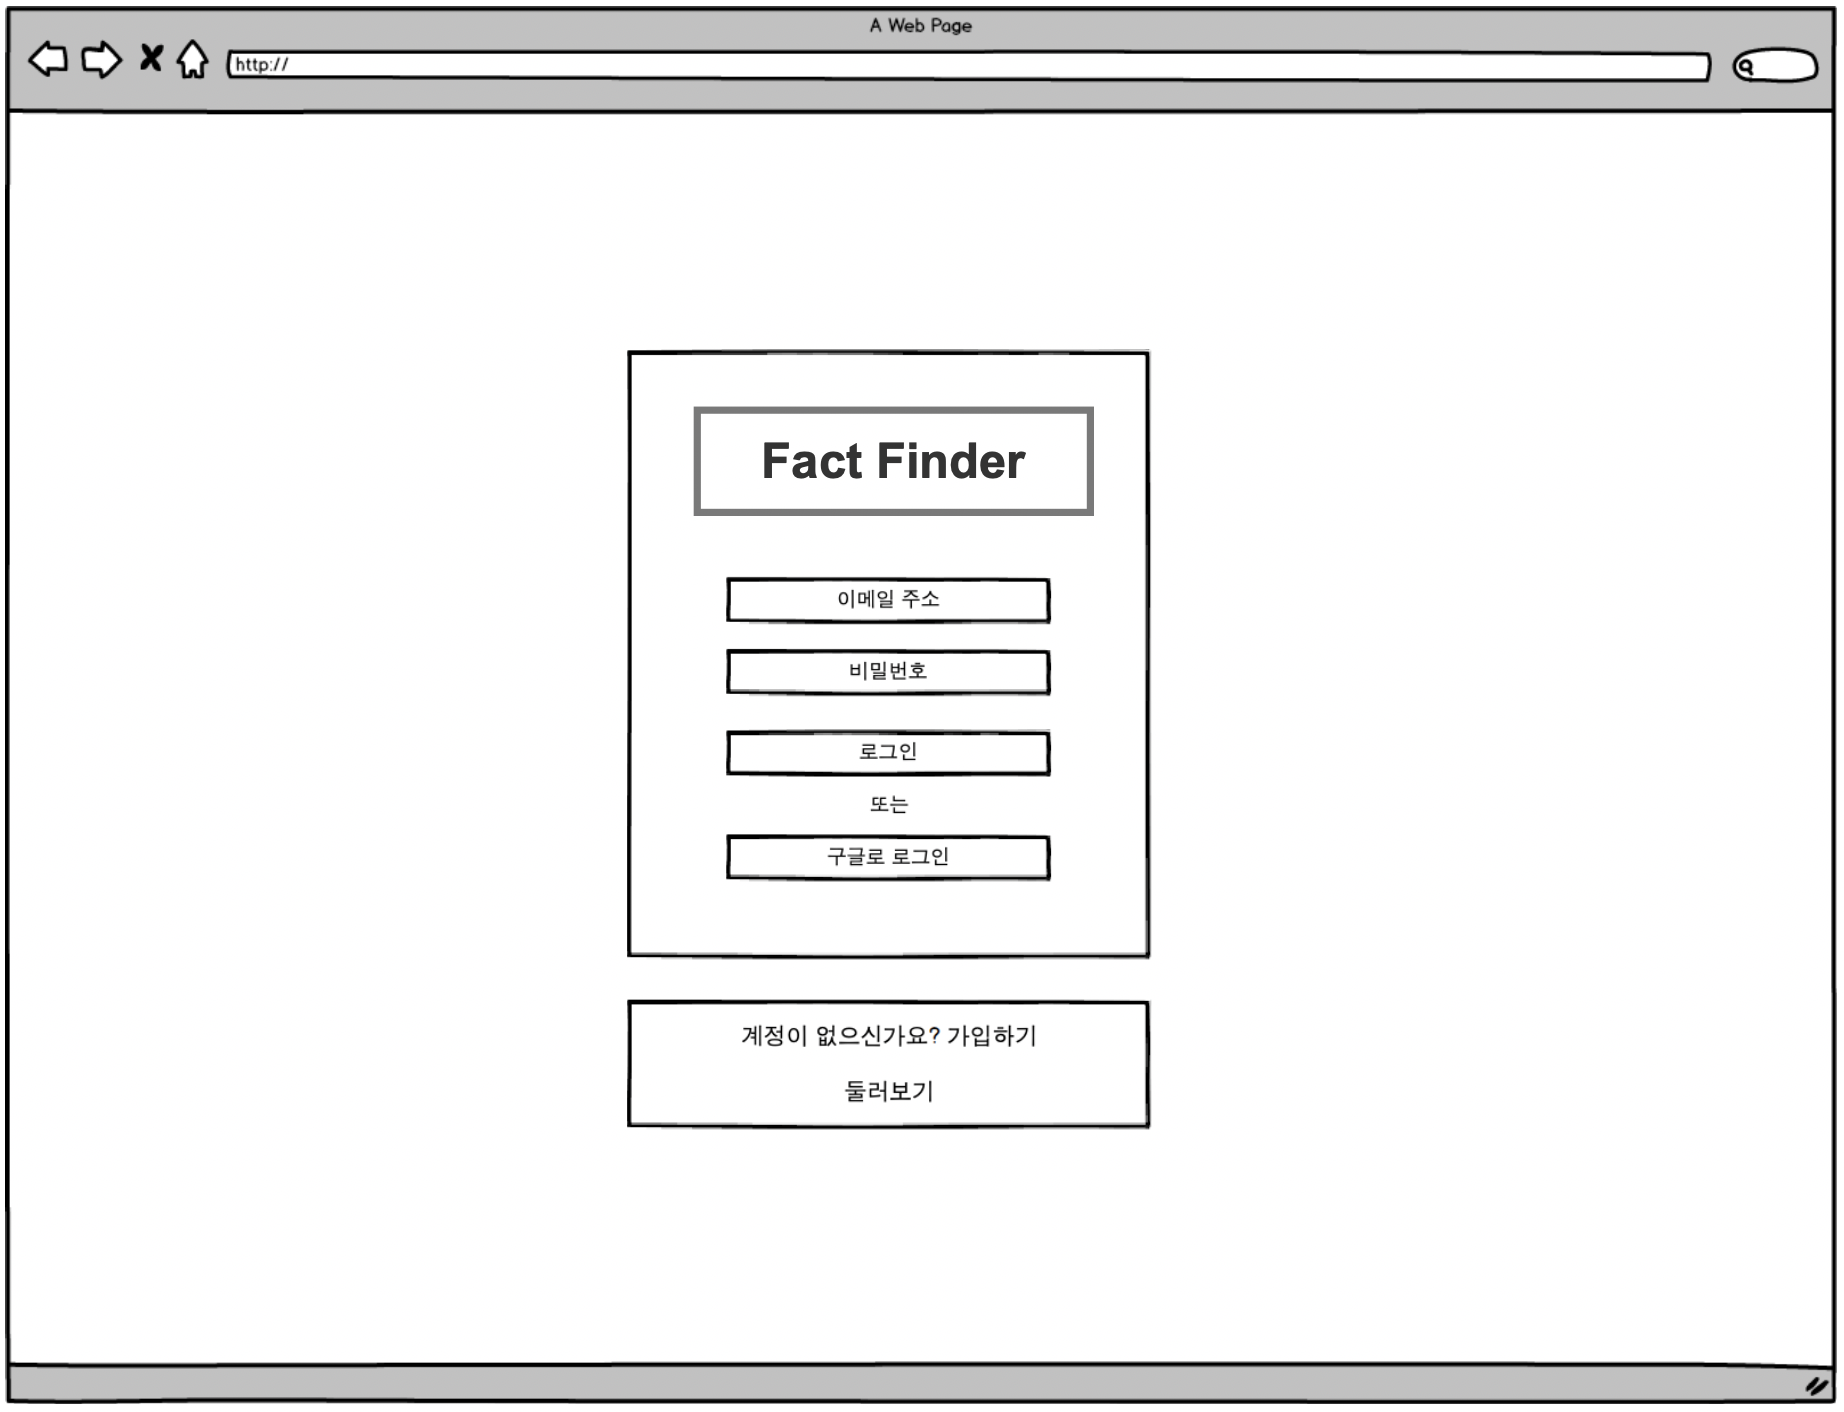
\includegraphics[width=89mm,scale=0.5]{fig/1.png}}
    \caption{Log-in}
    \label{fig}
    \end{figure}
        \item \textit{Log-in: }Log-in page is a first page that users can see when they enter to our website. The user have to fill out their e-mail and password in this page.  If username and password are match to our database, user can log in our web page to use our personalized system. If users succeed to log in, they can be identified through the internal identifying process so that they can move into the main page . Although, they bump into the failure message if the password is wrong. furthermore, if they enter wrong password  over five times, their accounts are locked so that they have to certificate their identity through contact address such as e-mail, phone number to get certification number to unlock their accounts.  If they want to use our service without login, they can press “looking around button”. In this case, they can use our service without our “subscribing function of interested politician. Also they can choose “Sign up button” to get into the sign up page  if they want to sign up to our service.\\
        \\
        \begin{figure}[htbp]
    \centerline{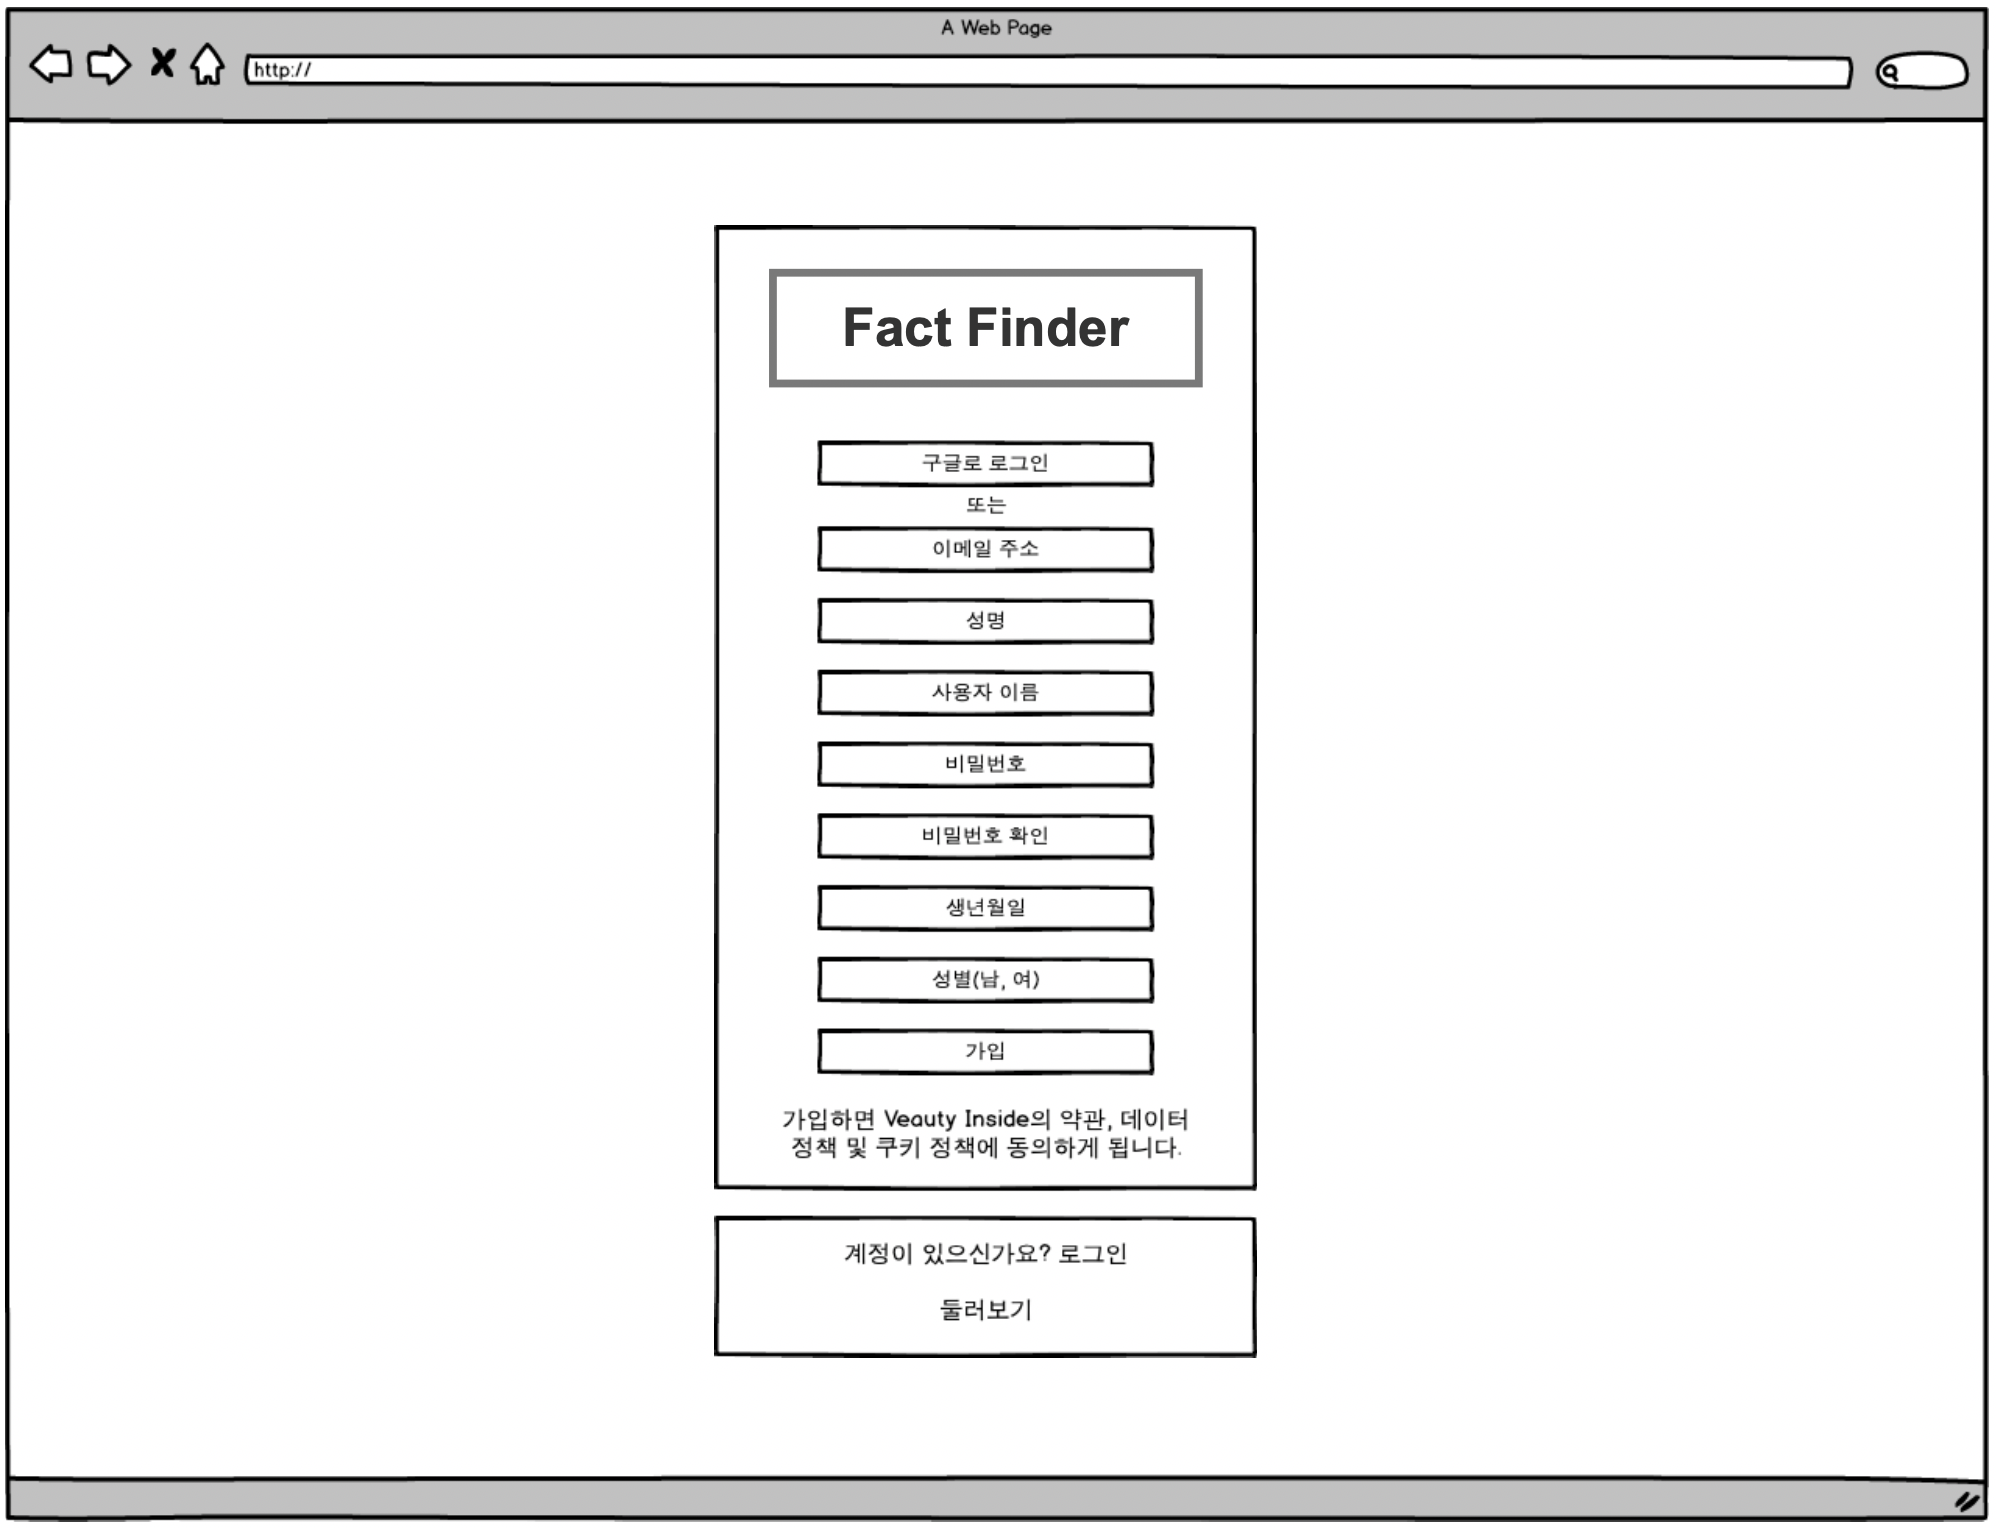
\includegraphics[width=89mm,scale=0.5]{fig/2.png}}
    \caption{sign-up}
    \label{fig}
    \end{figure}

        \item \textit{sign-up: }This page requires user to users’ information  such as E-mail, Username, Nickname, password, birth date, sex. These information are submitted to our database. Also, user must agree on our services’ terms, data, cookie policy. User can sign in into our page if they finish their forming information process. Furthermore, User can sign up through Kakao talk, Google, Naver ID certificating processes. If they want to use our service without login, they can press “looking around button”. In this case, they can't use our service without our “subscribing function of interested politician. Also they can choose “Sign up button” to get into the sign up page  if they want to sign up to our service.\\
         \item \textit{ID/PW search: }If the user forget about their ID or Password, they can find theirs through this page. Through the information saved on our database, user can certificate themselves by sending certification number to their E-mail,  phone number, or I-PIN. User should change their password after this function.\\
    \end{enumerate}
    
    \item \textit {Main Page: }
  
The main page is a key feature of this service. Users can search for detailed information about minutes. Service website is designed with simple and easy features because of users' readability of our letters. To concrete this, the following functions are implemented.\\

         \begin{enumerate}
    \item \textit{Basic components residing whole web-site:} It consists of website's basic components like Navigation bar that contains several link on whole web page and footer that contains subordinative information. Also, our web service's overall color concept is based on navy color. \\
            \begin{enumerate}
    \item \textit{Navigation bar:} it contains several components of the application and user can can navigate to the selected page by selecting the list. navigation bar consists of the following items and is linked to each item. This Navigation bar resides on our whole web page in under side to make our user link in  whole web site easily. It's links consists of to all of our core web function, "1. Looking up list of assembly minutes, 2. Looking up list of agendas per specific assembly minutes, 3. Looking up dialogue of specific agenda, Looking up function about agenda participating specific politicians, 4. Looking up function about politician's speech according to agenda, 5. Looking up function about subscribing politicians, 6. Searching real speech of the politician function" \\
    
    \item \textit{Footer:} It consists of our team location, contact numbers, email, Legal information, Official SNS links, related website. It resides on our whole web page in upper side to make our user see our team information easily.
    \\
        \end{enumerate}
            \end{enumerate}
    
    \begin{enumerate}
        \item \textit{Looking up function about meeting contents per agenda:} This function consists of three pages, Looking up list of assembly minutes, Looking up list of agendas per specific assembly minutes, Looking up dialogue of specific agenda.
        \\
        
         \begin{enumerate}
         
    \begin{figure}[htbp]
    \centerline{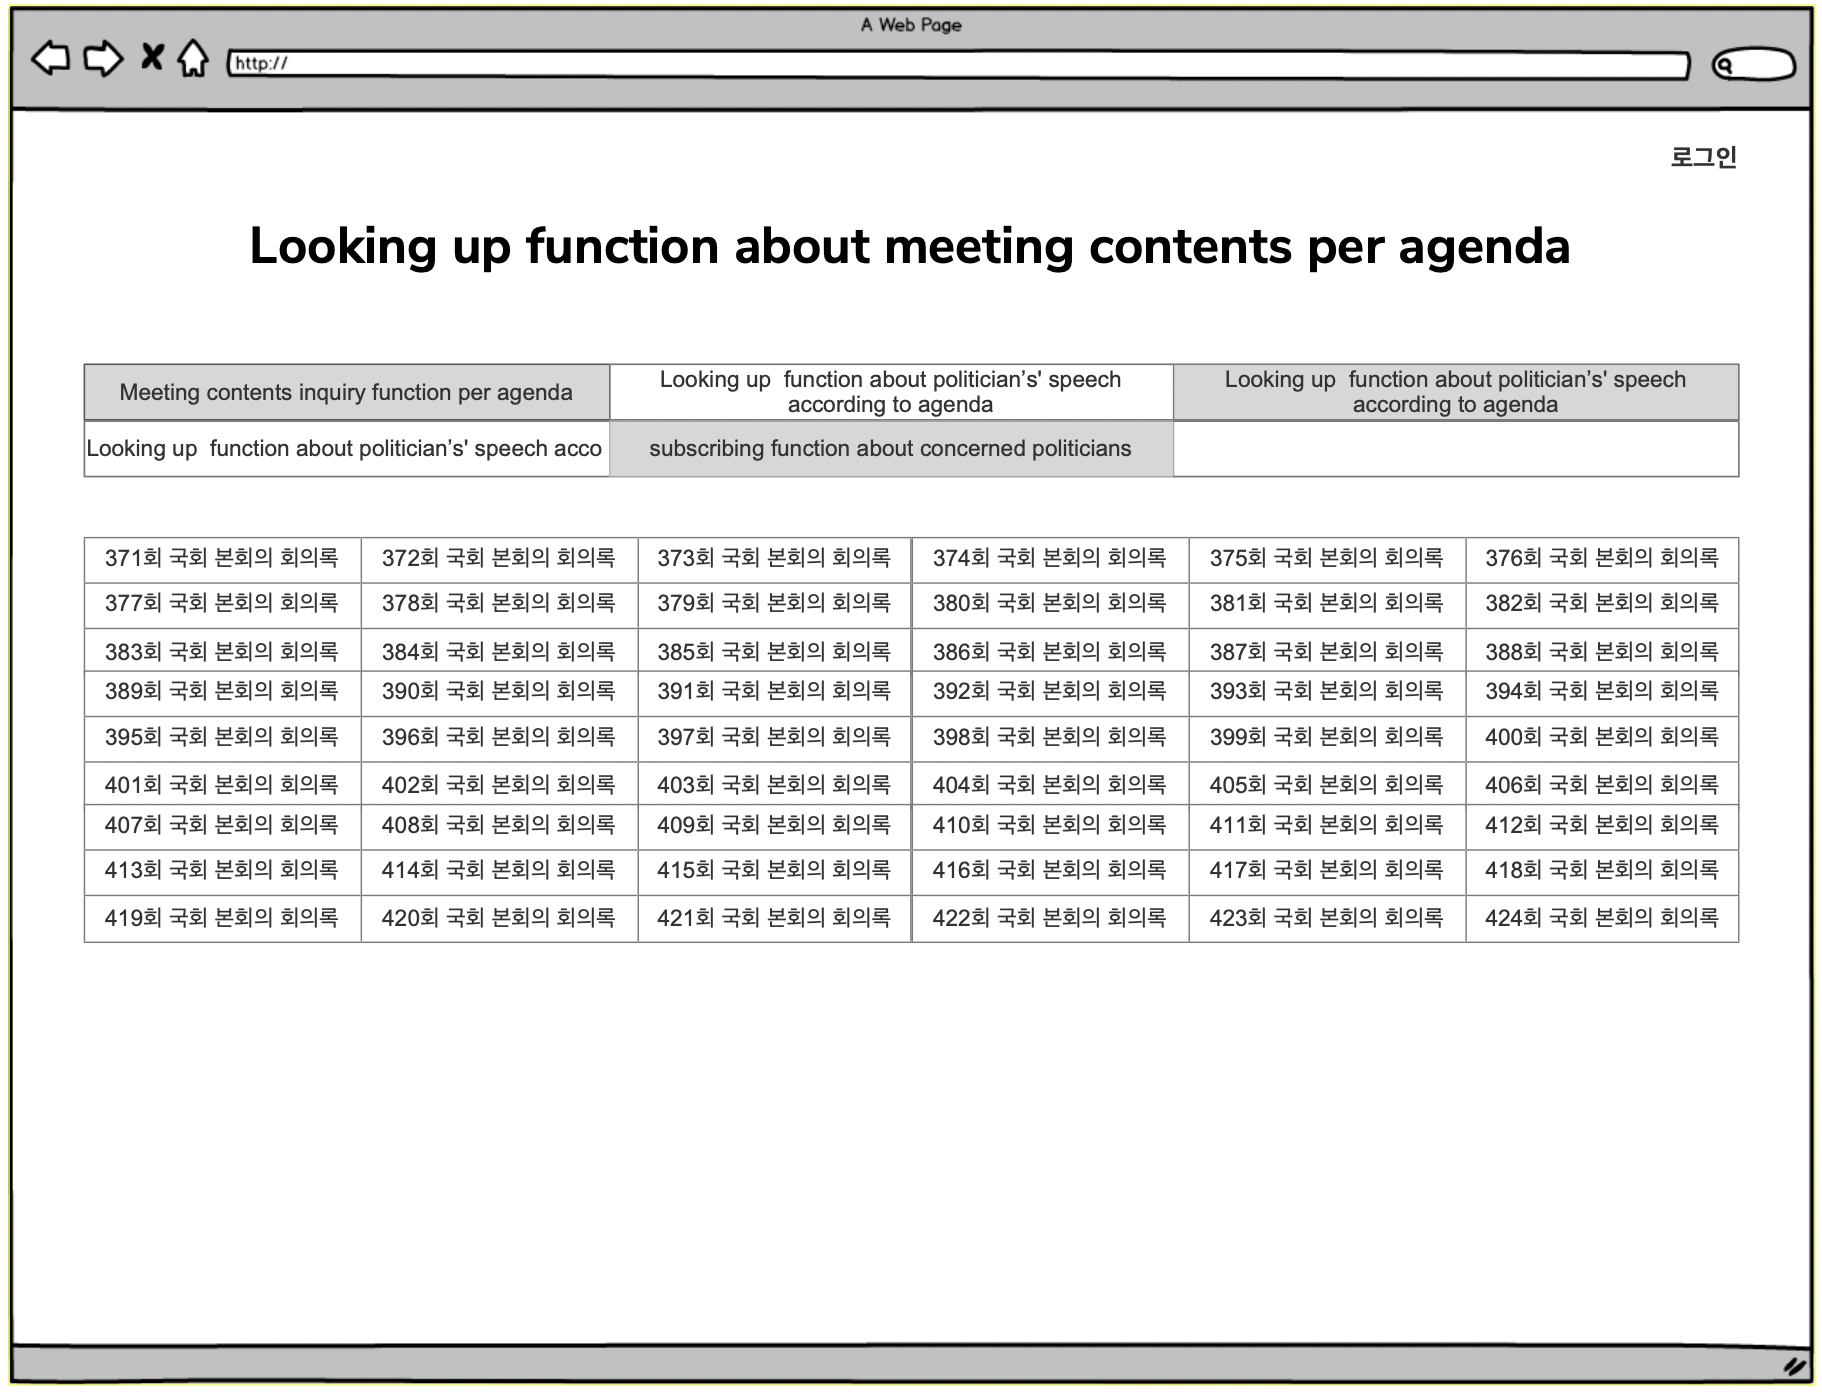
\includegraphics[width=89mm,scale=0.5]{fig/3.png}}
    \caption{Looking up list of assembly minutes}
    \label{fig}
    \end{figure}     
        \item \textit{Looking up list of assembly minutes:} In first page, it shows assembly minutes list. Minutes list that is classified periodically includes monthly, weekly, and certain time period setting function. Because of this, user can search the record of the past and view minutes in certain date. The minutes are classified by kinds of minutes. The kinds are like, "The main session of state affairs, standing committees, special committees, confirmation hearings, subcommittees, parliamentary audits, public hearings, hearings and joint meetings". If the amount of list in single page is too many(up to 50), this page is paginated to next page.\\
    
        \begin{figure}[htbp]
    \centerline{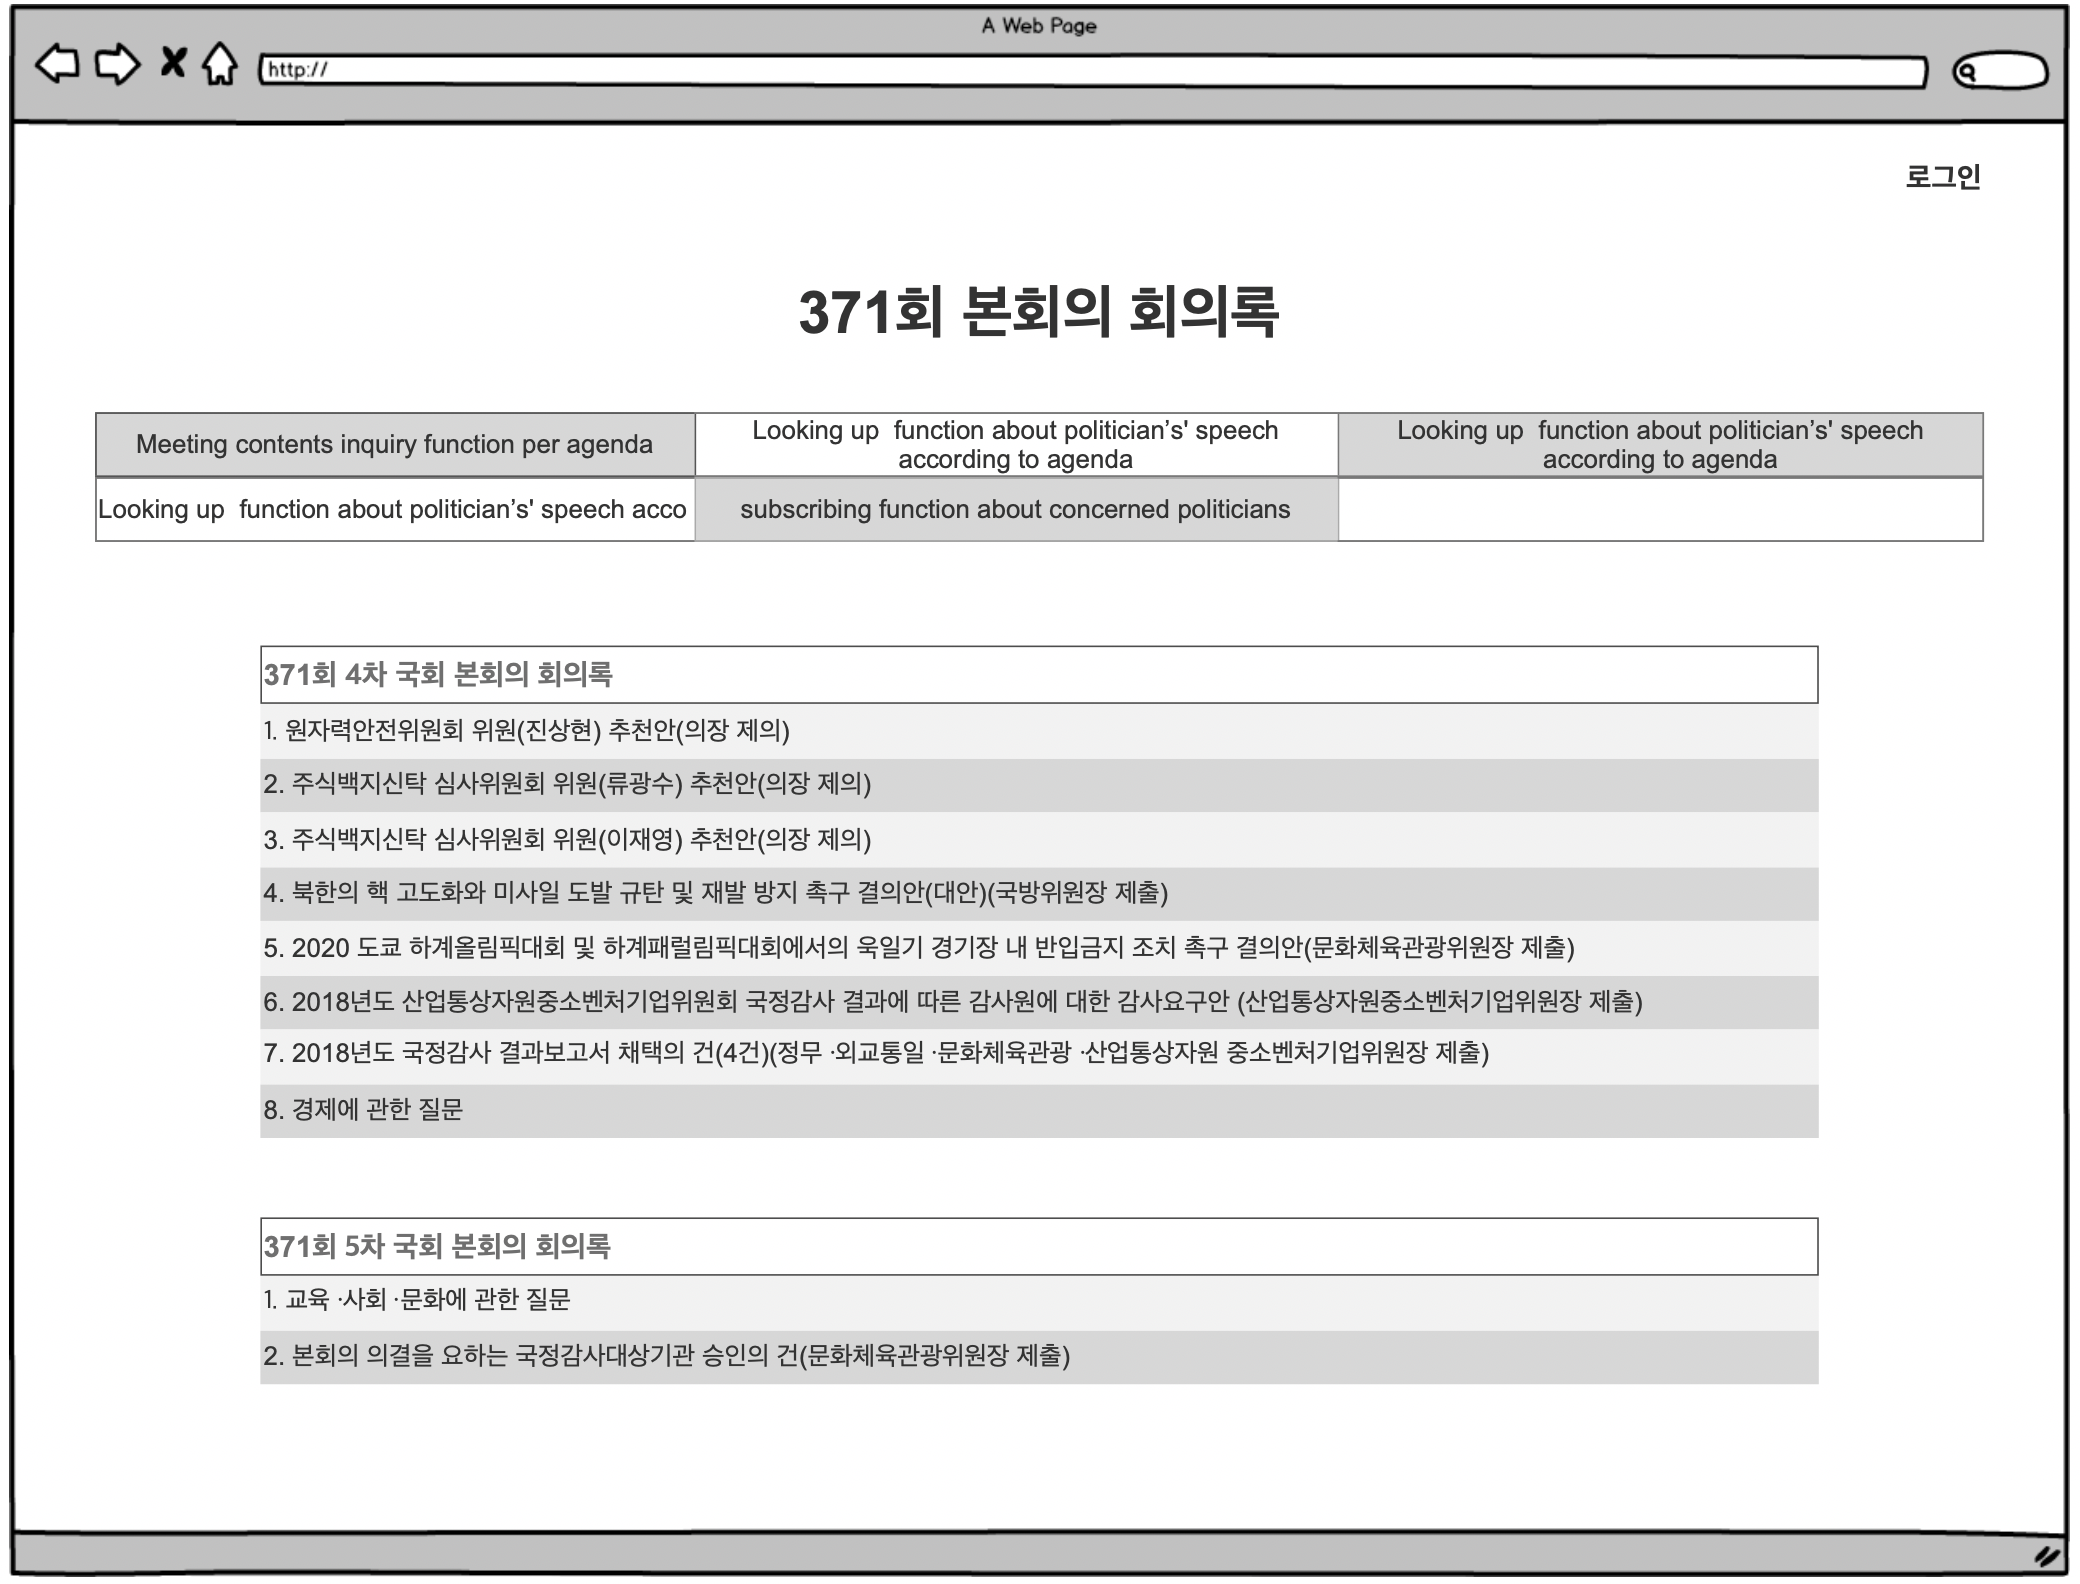
\includegraphics[width=89mm,scale=0.5]{fig/4.png}}
    \caption{Looking up list of agendas per specific assembly minutes}
    \label{fig}
    \end{figure}     
    
        \item \textit{Looking up list of agendas per specific assembly minutes: } In Second page, It consists of each minutes’ count number and agendas. In the big table, it shows each count number, specifically, each table contains what agendas are discussed in that congress meeting. If user wants to search specific agenda, he can just view that  by clicking that agenda. He can move onto the detail page. This page can be basically scrolled down, but, If the amount of list in single page is too many(up to 10), this page is paginated to next page.\\

                \begin{figure}[htbp]
    \centerline{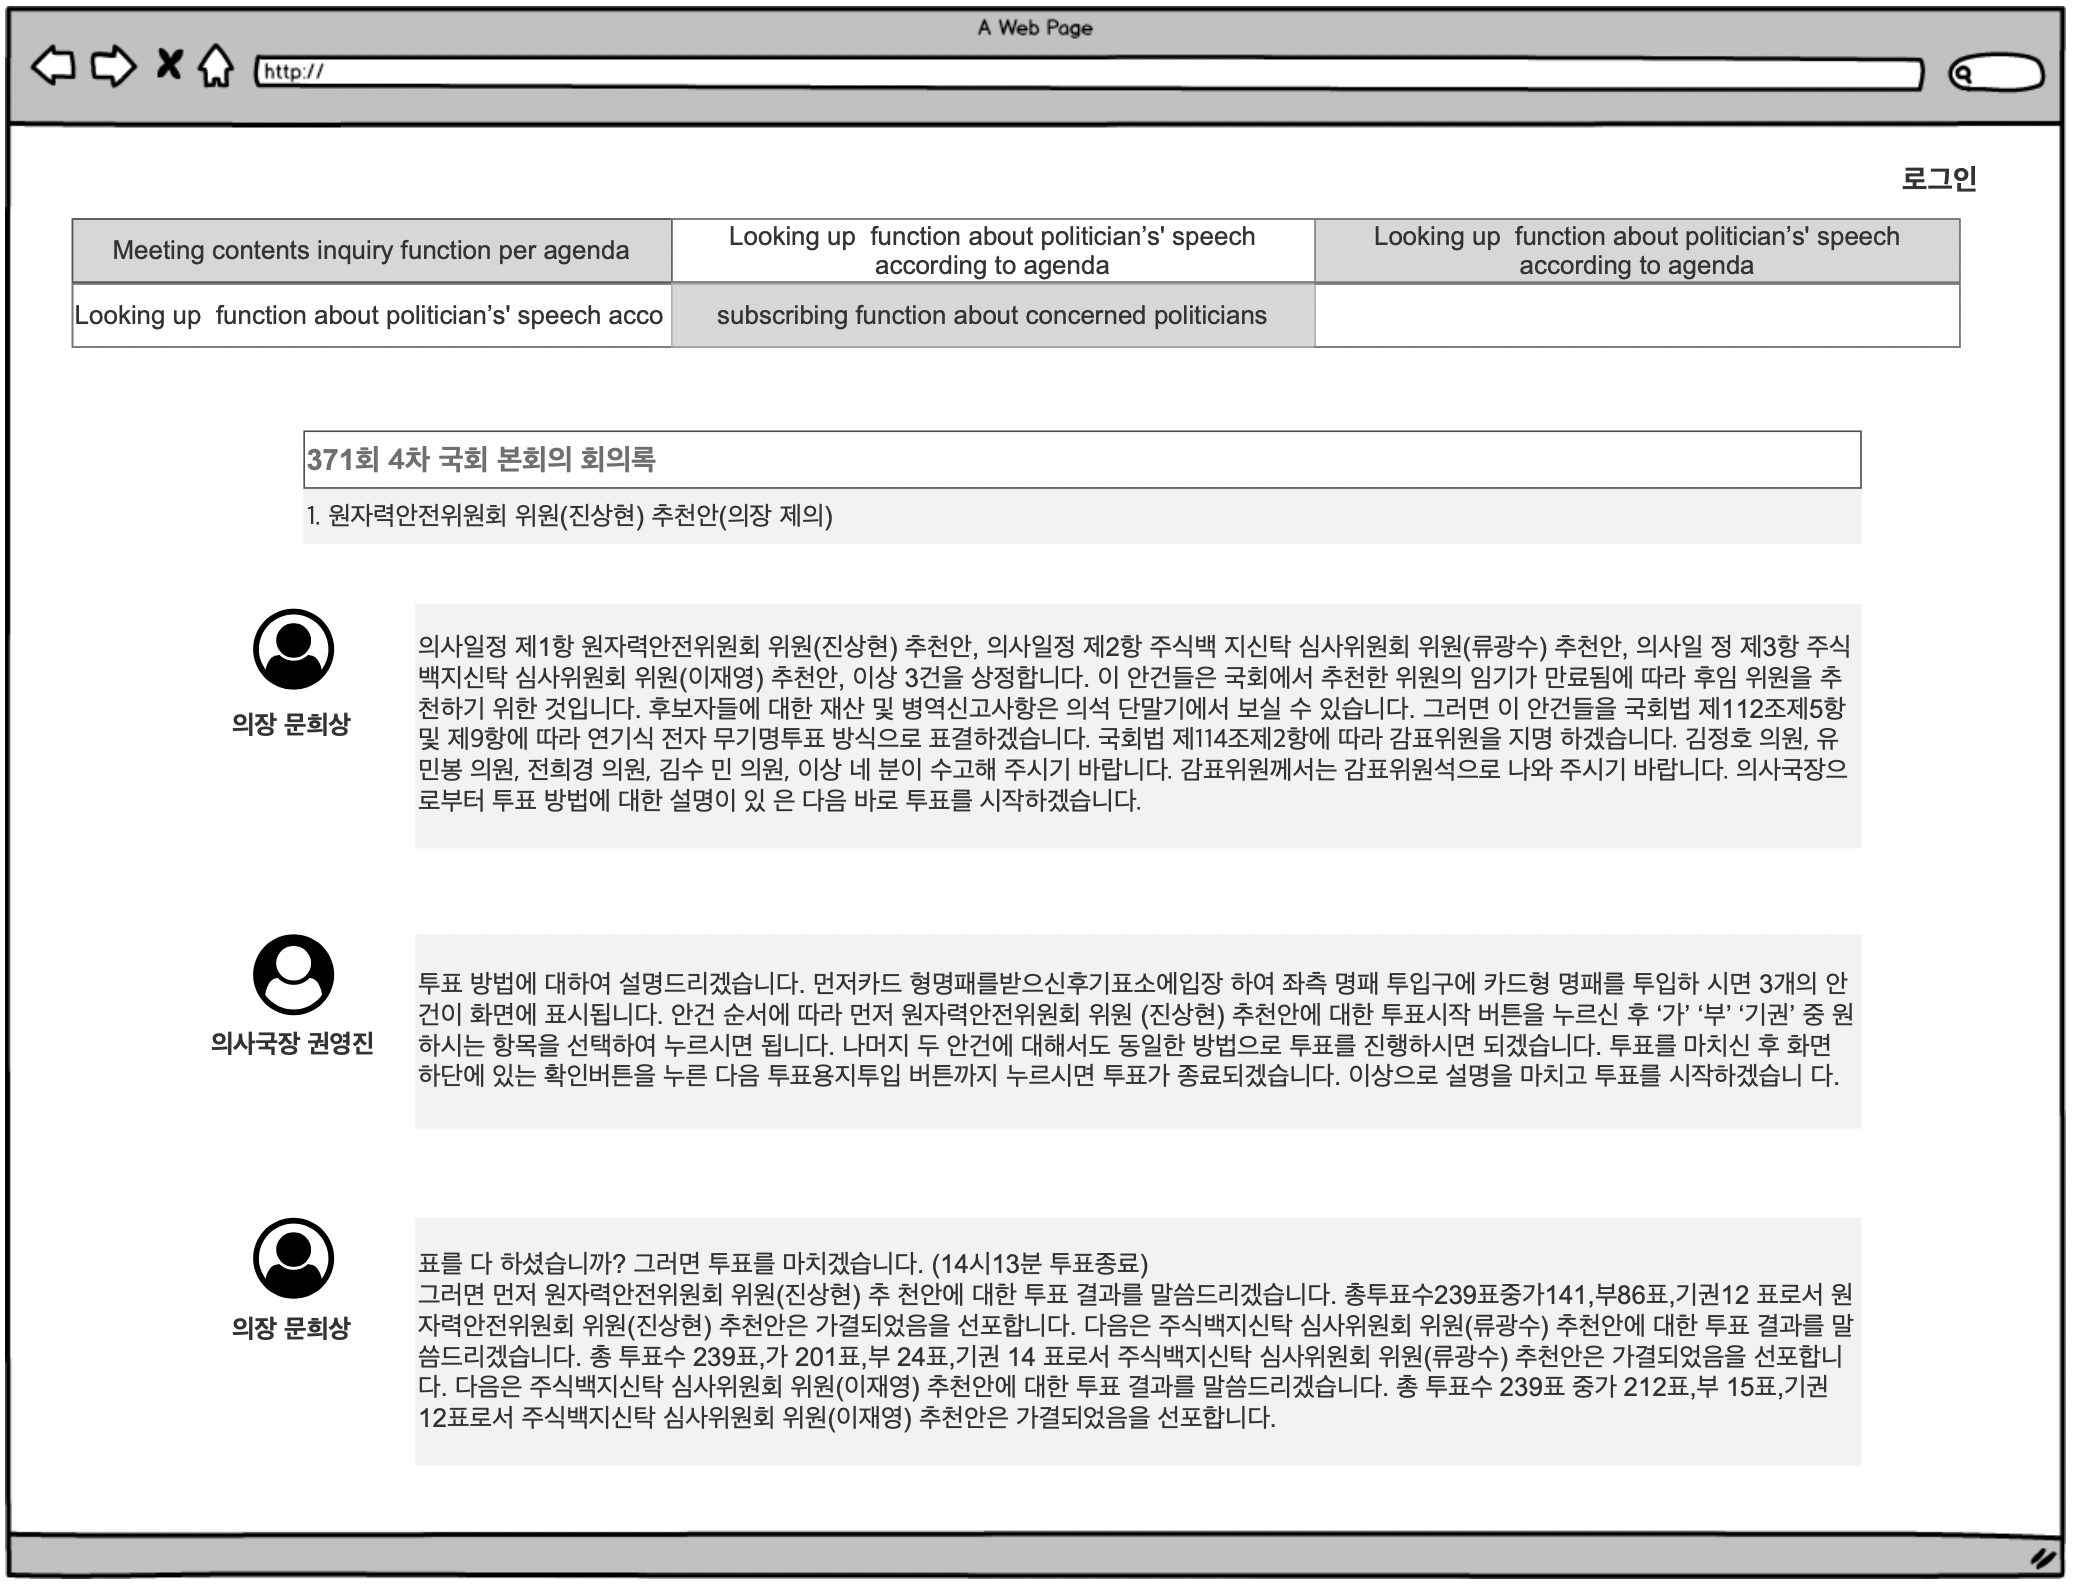
\includegraphics[width=89mm,scale=0.5]{fig/5.png}}
    \caption{Looking up dialogue of specific agenda}
    \label{fig}
    \end{figure}     

         \item \textit{Looking up dialogue of specific agenda: } In third page, it shows detail page that belonged to chosen agenda by the user. It looks like social messenger, talking each other like shown above. Specifically, The politician’s image is attached and his or her speech is surrounded in a box. One single page is not finish until specific agenda is over.\\
           \end{enumerate}
               \vspace{60mm}

                        \begin{figure}[htbp]
    \centerline{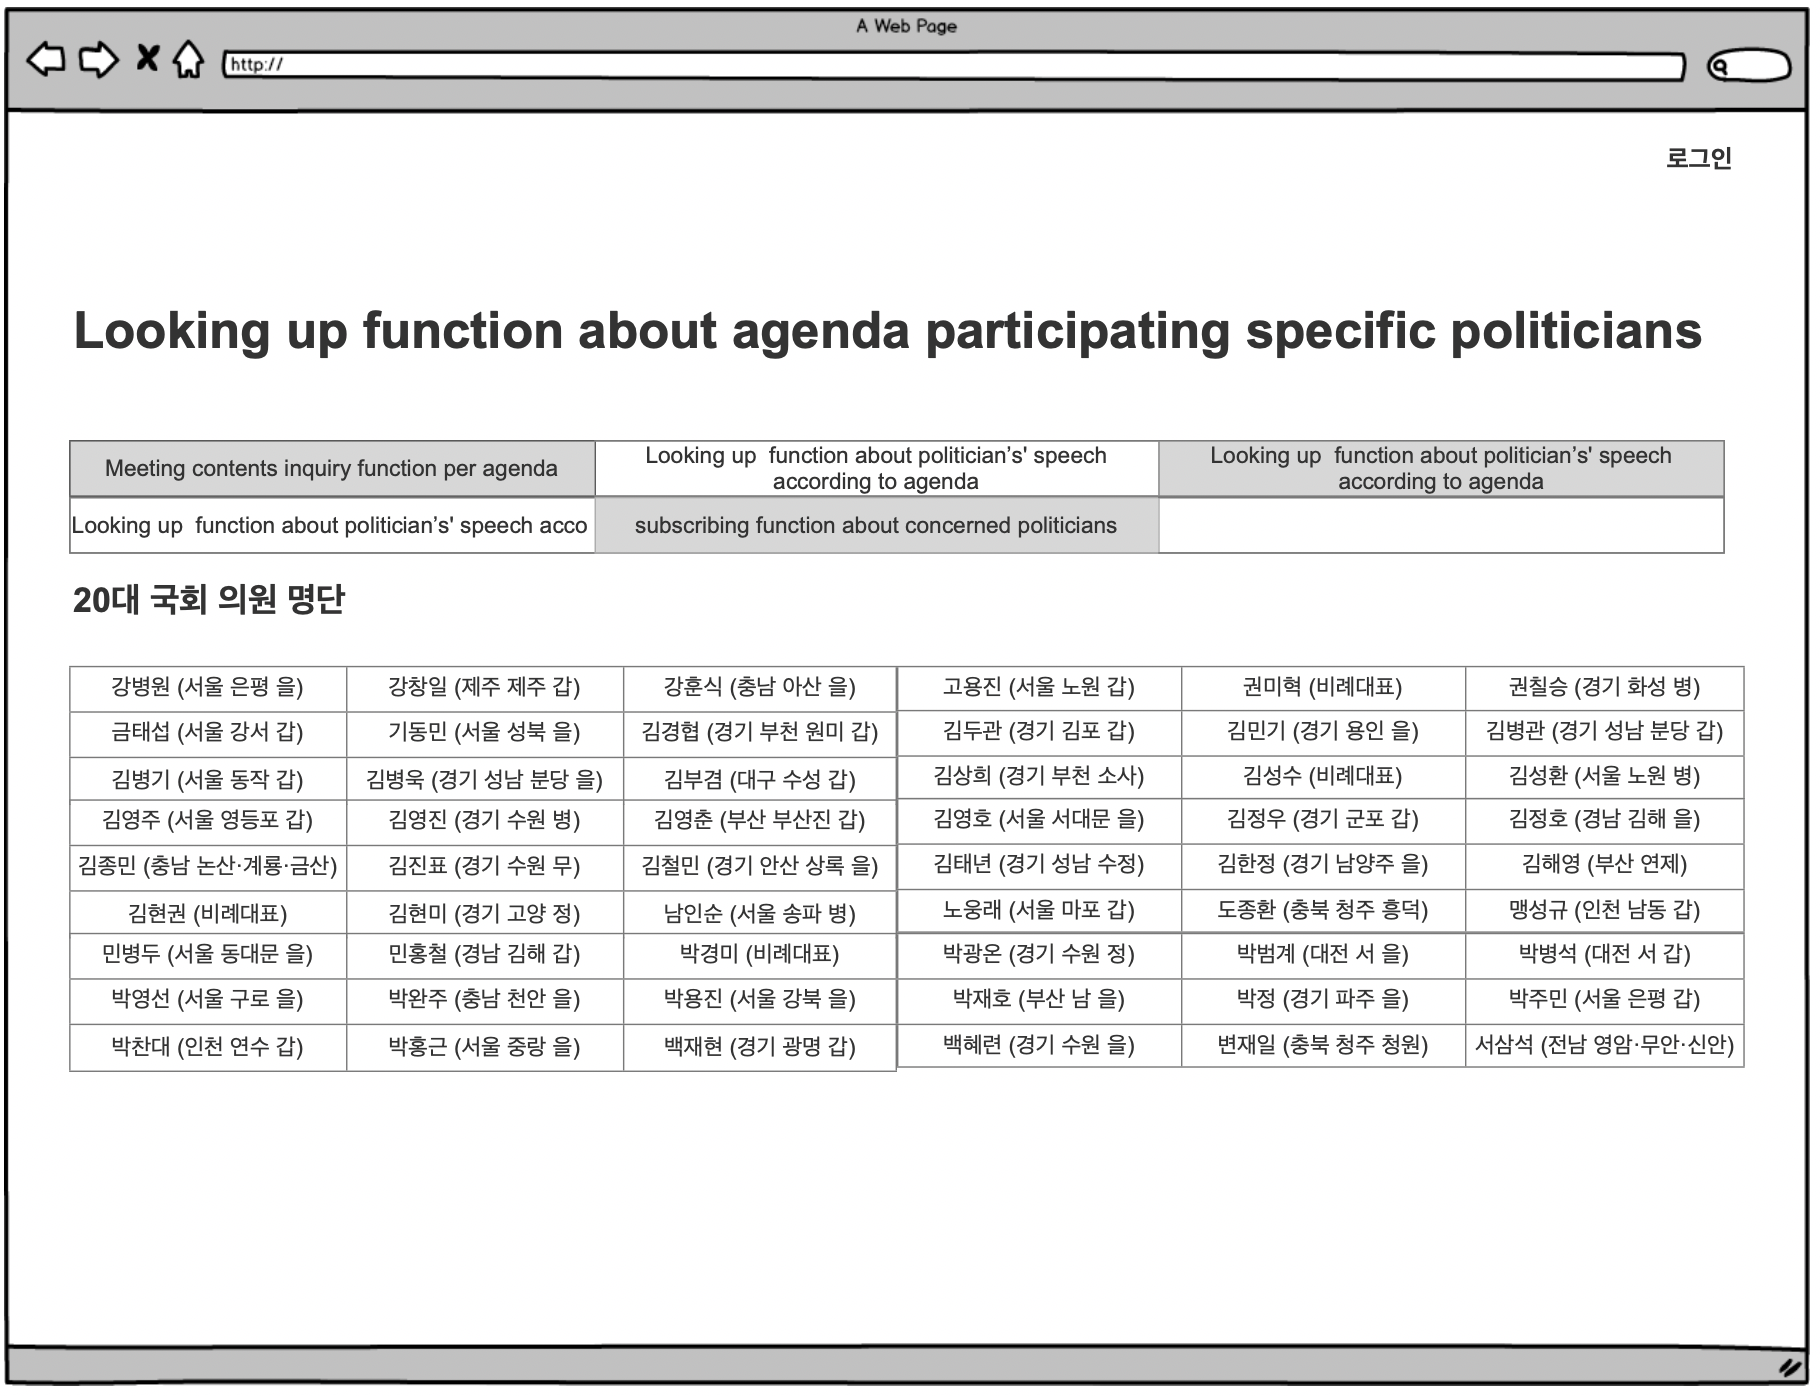
\includegraphics[width=89mm,scale=0.5]{fig/6.png}}
    \caption{Looking up function about politician list}
    \label{fig}
    \end{figure}     

        \item \textit{Looking up function about politician list: }  \\
                 \begin{enumerate}
 
        \item \textit{} In this page, user can view politician list. User can view current members of assembly along with where they are belonged to. If user click a member, they can move onto the page that politician’s commented agendas. in other words, This page is connected to as a separated function as third below, “Looking up  function about politician’s speech according to agenda”. \\
        \item \textit{Subscribing function about interesting politicians:} If user wants to follow specific politician what they did in assembly  on and on, they can click subscribe button in the member box. In this case, user can check what they saved in the fourth function, “Looking up function about subscribing politics”. This function is activated only if the user was logged in.\\
           \end{enumerate}
              \vspace{57mm}

                                    \begin{figure}[htbp]
    \centerline{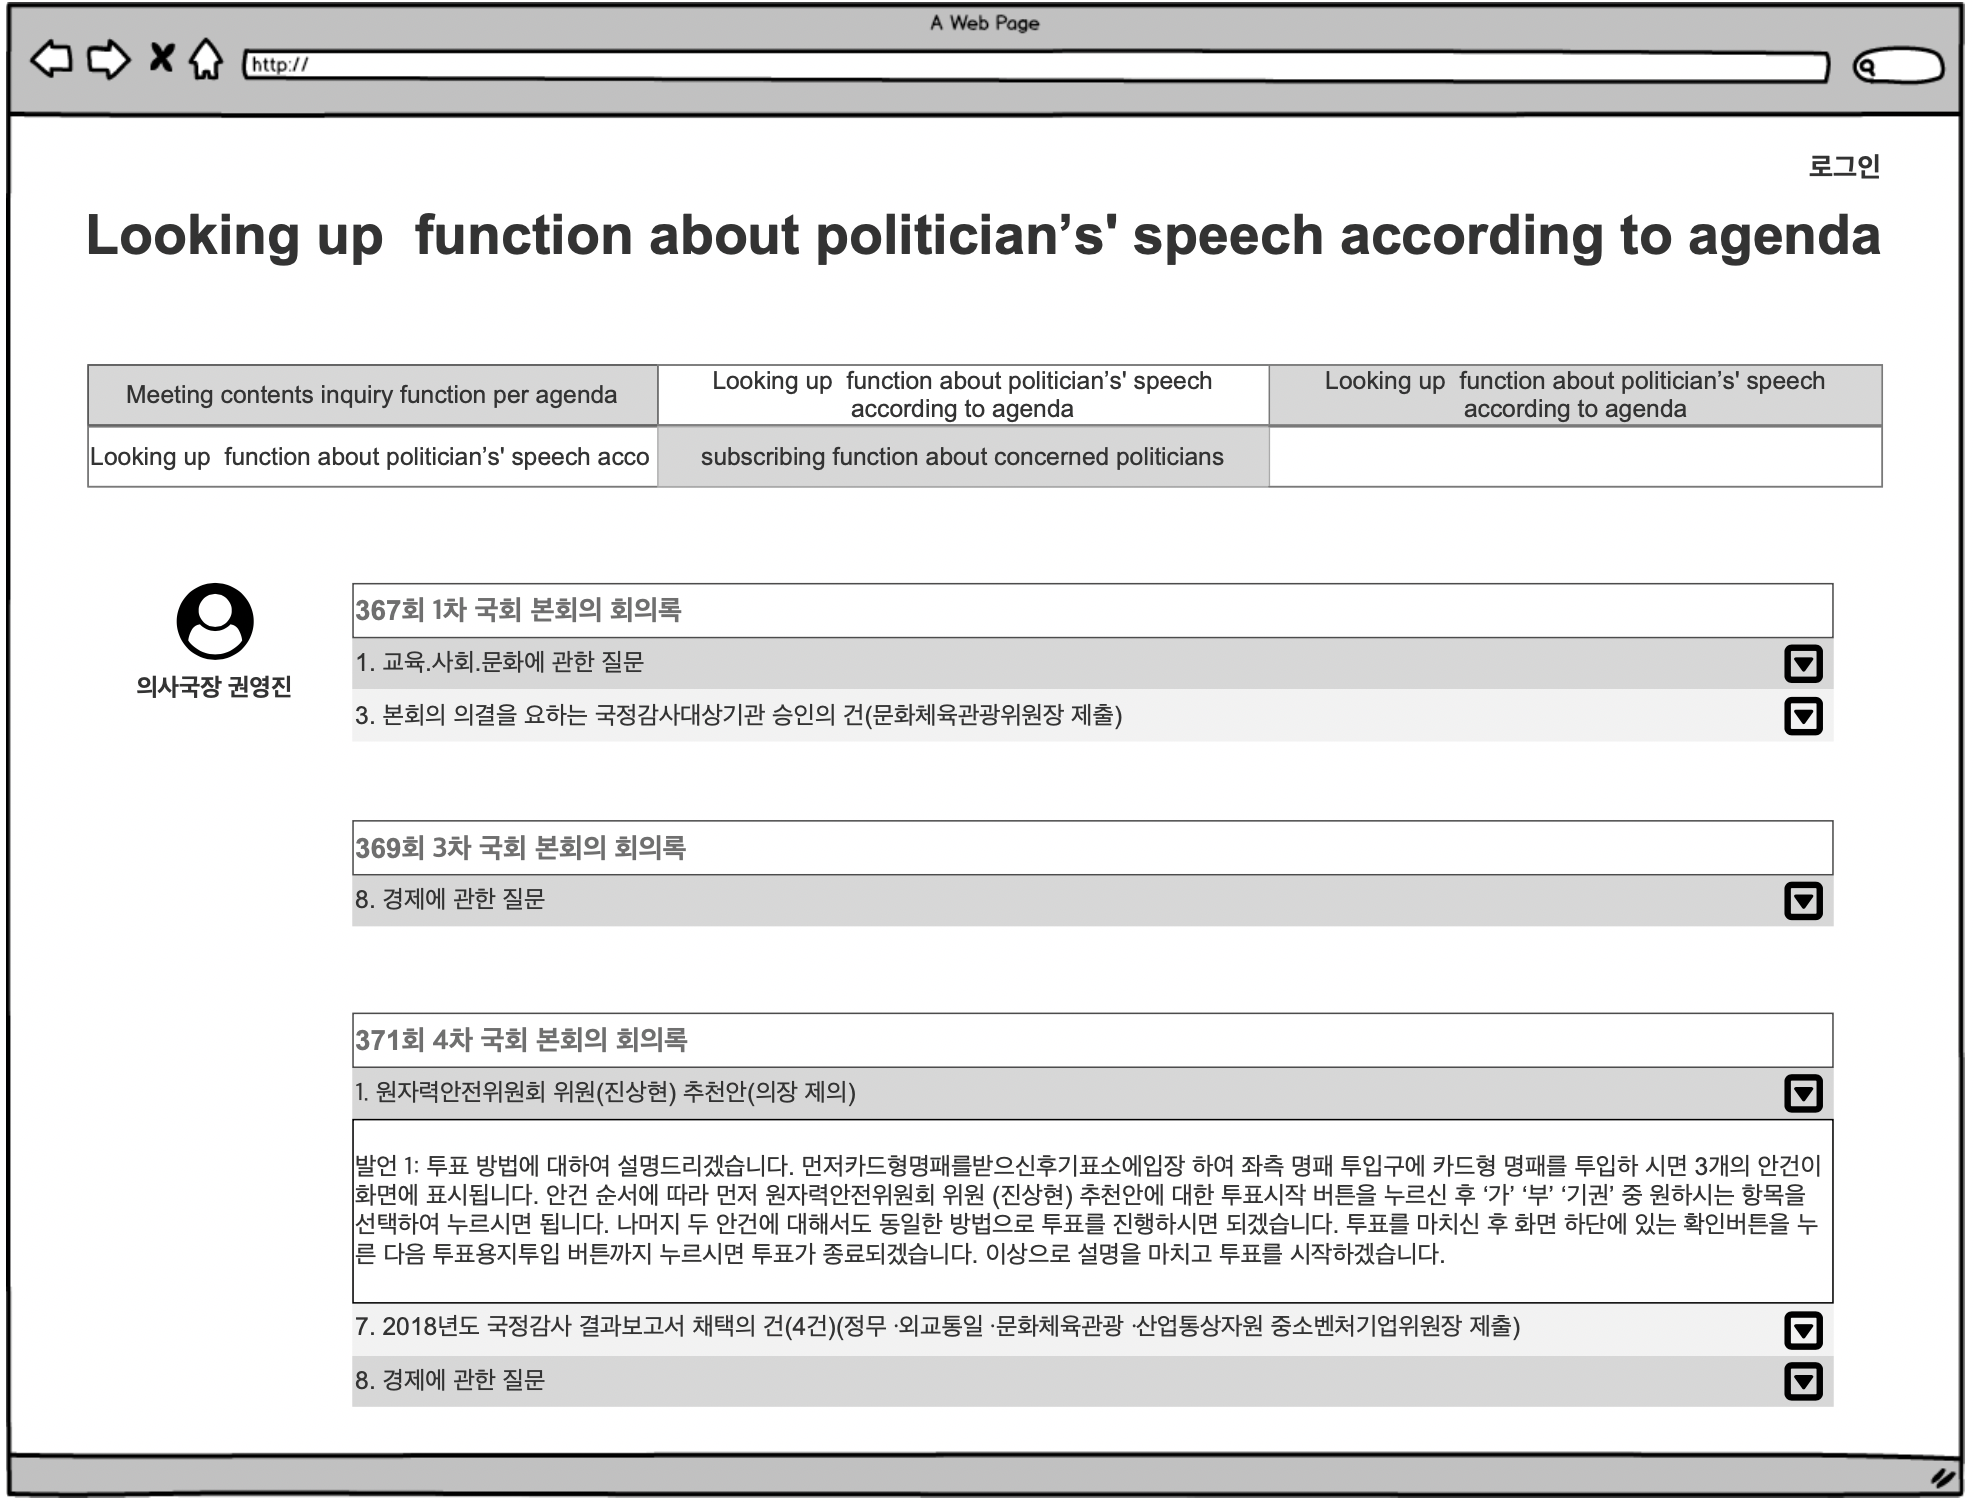
\includegraphics[width=89mm,scale=0.5]{fig/7.png}}
    \caption{Looking up  function about politician’s' speech according to agenda}
    \label{fig}
    \end{figure}     

        \item \textit{Looking up function about politician’s speech according to agenda:}  \\
                 \begin{enumerate}
 
        \item \textit{} If user selected or searched to specific politician, they can view this page. In this page, User can see specific politician’s participated agenda. Each table is consisted of the name of the assembly minutes, and details are filled with that politician’s participated agenda. If user wants to view what they spoke specifically at that agenda, they can click the pointing down arrow button. the pop-up box shows the politician’s speech, and its contents are separated with numbers like ‘speech1, speech2’.\\
        \item \textit{Subscribing function about interesting politicians: } If user wants to follow specific politician what they did in assembly  on and on, they can click subscribe button in the member box. In this case, user can check what they saved in the fourth function, “Looking up function about subscribing politics”. This function is activated only if the user was logged in.\\
           \end{enumerate}
         \vspace{40mm}

               \begin{figure}[htbp]
    \centerline{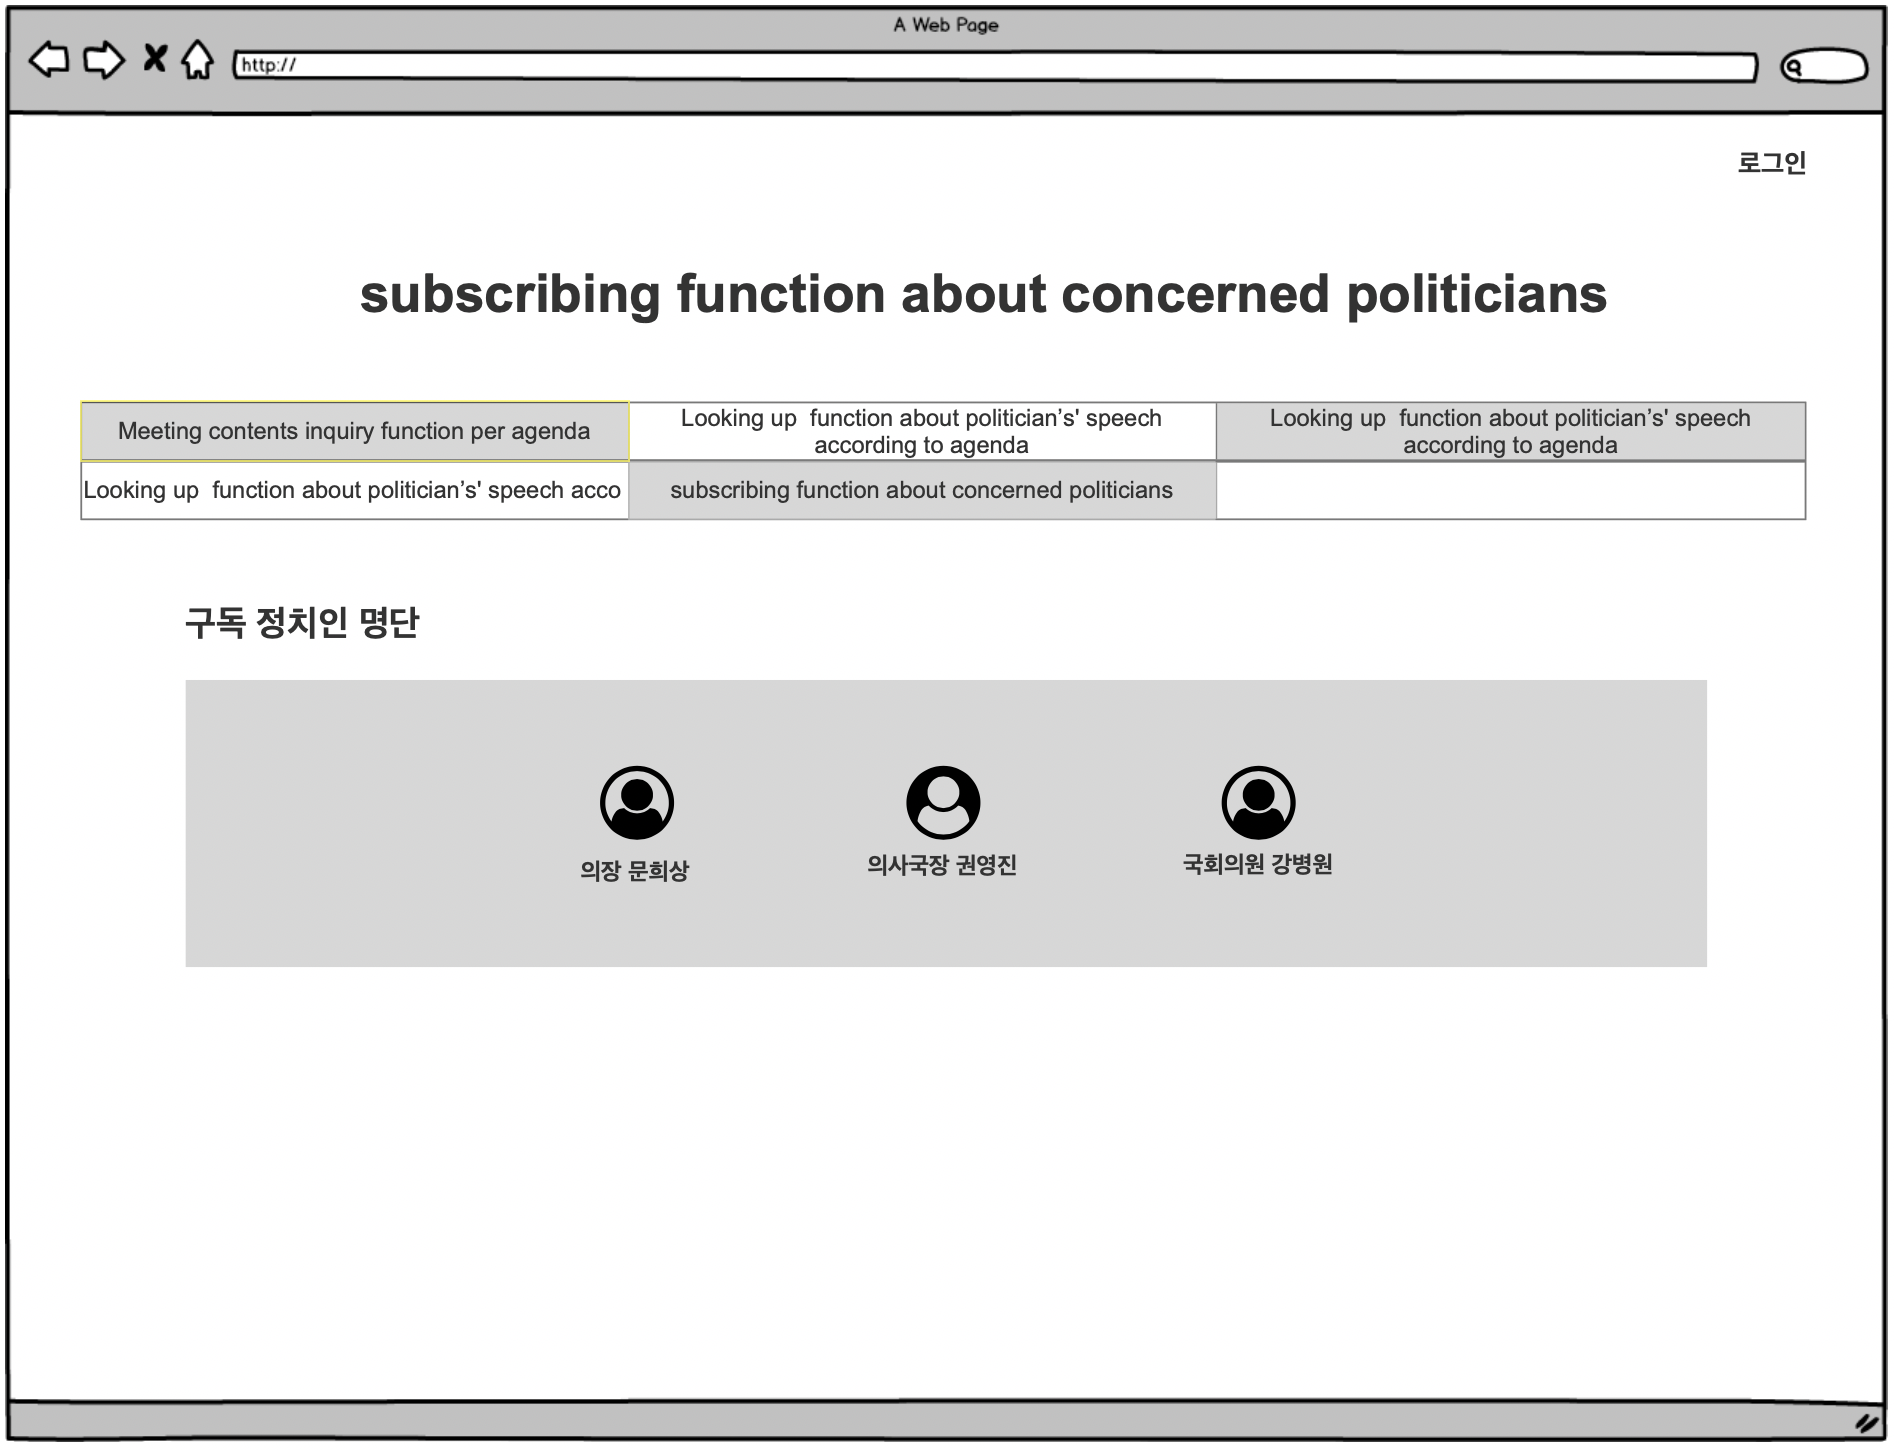
\includegraphics[width=89mm,scale=0.5]{fig/8.png}}
    \caption{Looking up function about subscribing politicians}
    \label{fig}
    \end{figure}     
    \item \textit {Looking up  function about subscribing politicians: }User can subscribe user’s interested politicians. In this page, user can customize this page by subscribing specific politicians functions implemented above. They can choose their favorite politicians. If the user click the image of politician, they can move onto the third function, “Looking up  function about politician’s' speech according to agenda”.\\
    
                                        \begin{figure}[htbp]
    \centerline{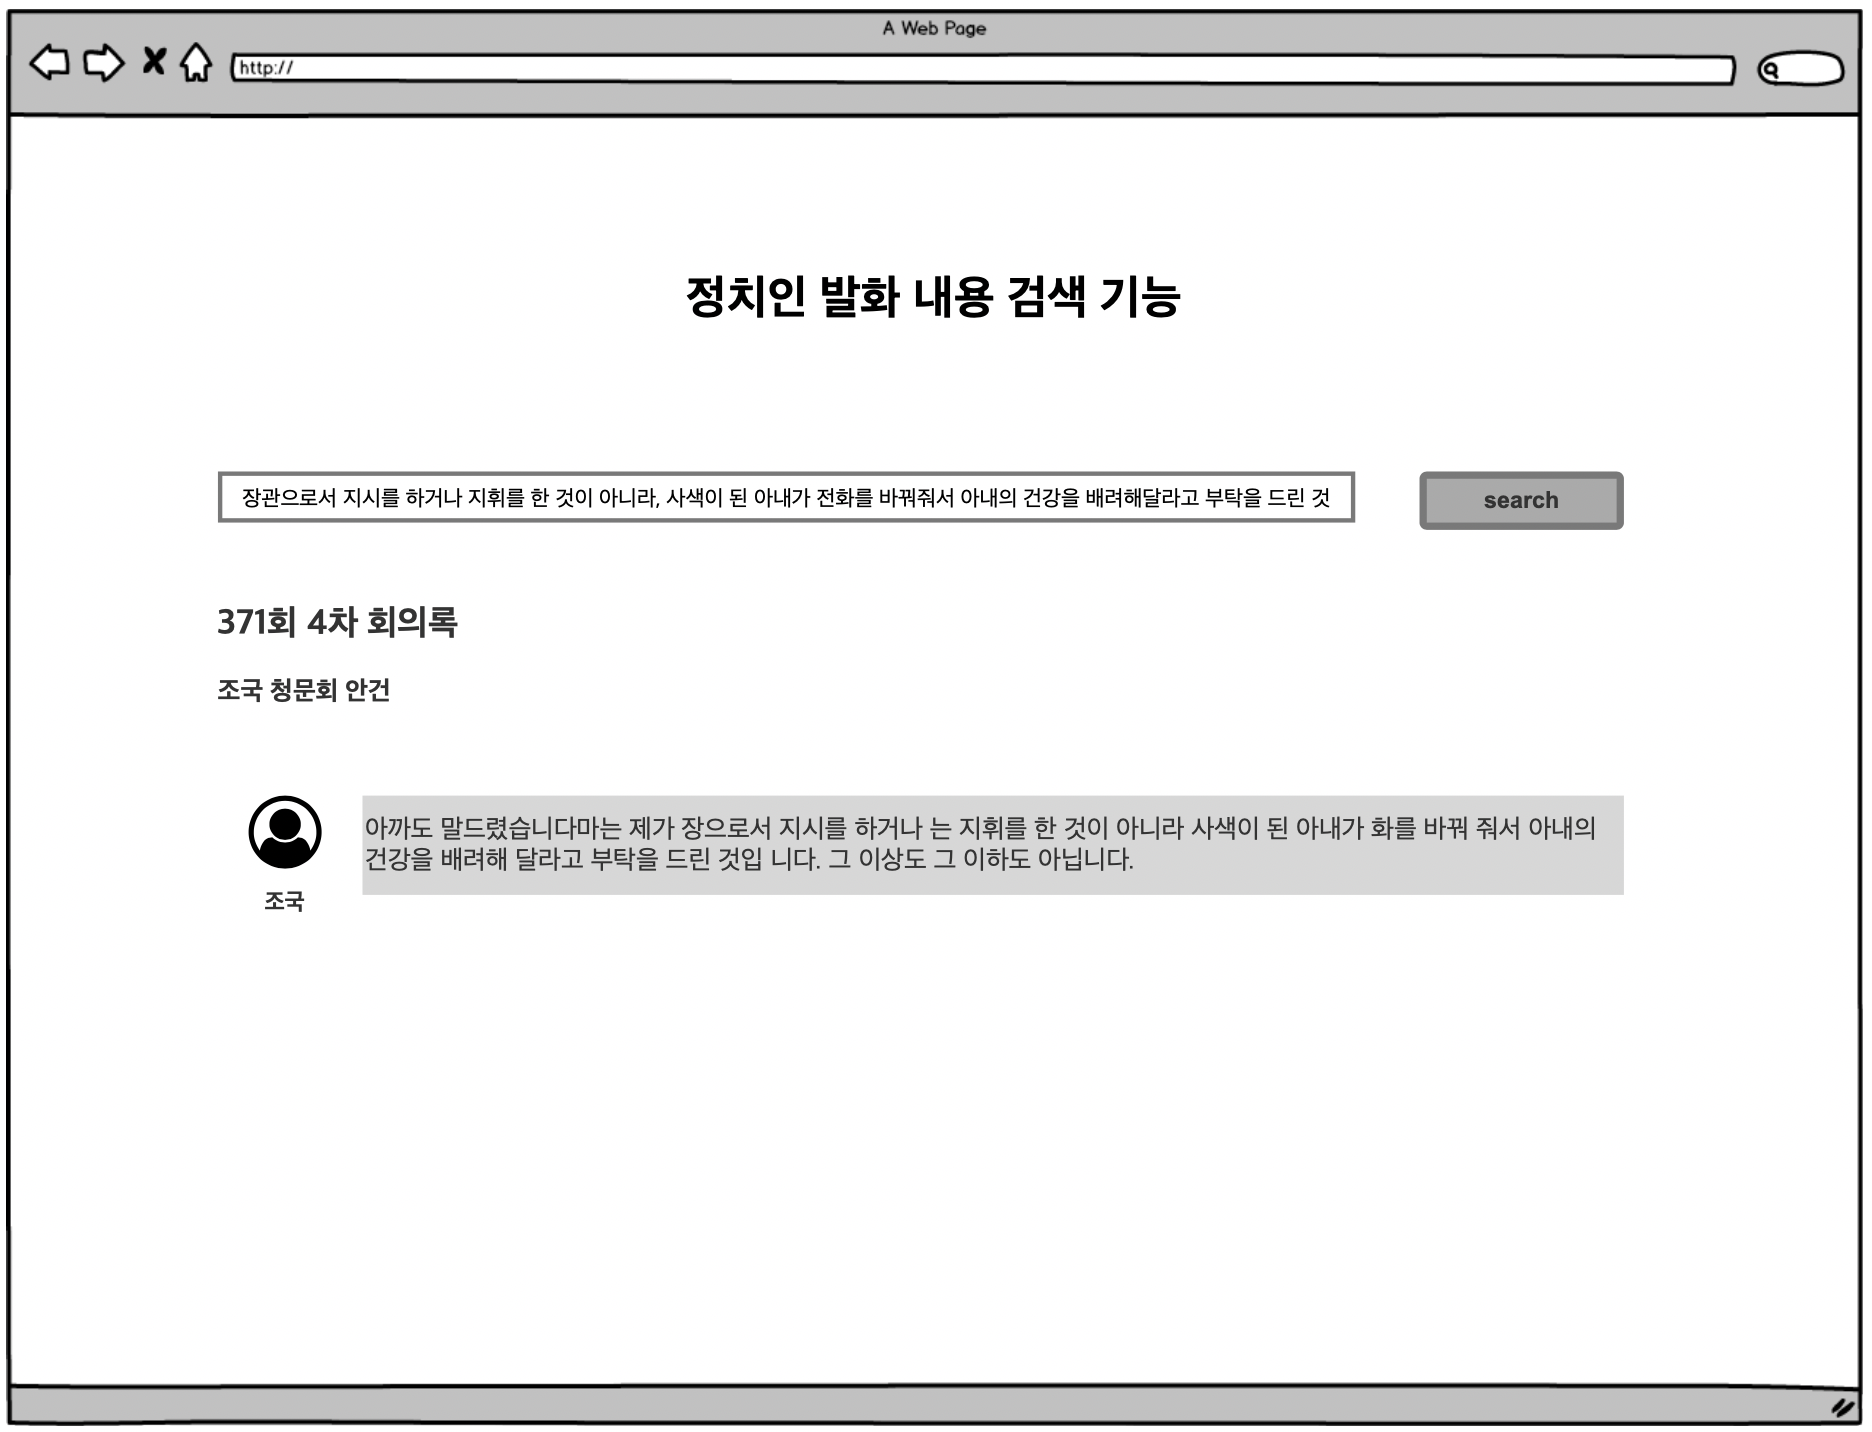
\includegraphics[width=89mm,scale=0.5]{fig/9.png}}
    \caption{Searching real speech of the politician function}
    \label{fig}
    \end{figure}     
        \item \textit {Searching real speech of the politician function: }This page is useful if the user wants to judge article’s quotation is true or not. User can search the facts in the minutes data, by filling out the search bar. If the user copy quotation in the article and paste in the search bar, they can click the search button. If then, what the politician actually said is popped out below with name of the assembly minutes, and agenda when he said at.\\
        \end{enumerate}
     
        \item \textit{Nugu service:} User can use our service through Nugu speaker. They can input specific utterance and the Nugu speaker answers back to the users. Searching information of the politicians, Looking up real speech of the politician in that agenda, Changing real speech of the politician in that agenda, Subscribing, Deleting about interesting politicians are should be implemented. This service is based on our database to be synchronized with our web service. 
            

        
\begin{table}[htbp]
  \renewcommand{\arraystretch}{1.5}
\caption{General Service Flow}
\begin{center}
\begin{tabular}{|p{1cm}|p{8cm}|}
\hline
\textbf{Speaker} & \textbf{Utterance}\\
\hline
User & Aria, tell me politician list that I subscribed. \\
\hline
Nugu & You subscribed [Politician1], [Politician2], [Politician3]. \\
\hline
User & Aria, tell me [Politician]'s (recent) participated meeting.\\
\hline
Nugu & [Politician] was participated in National Assembly [0th] conference.\\
\hline
User & Aria, tell me [Politician]'s (recent) participated agenda. \\
\hline
Nugu & [Politician] was participated in [agenda].\\
\hline
User & Aria, tell me [Politician]'s (recent) utterance.\\
\hline
Nugu & [Politician] said, "~~~".\\
\hline
\end{tabular}
\label{tab2}
\end{center}
\end{table}
        
\begin{enumerate}
        \item \textit{Searching information of the politicians function:} This function can search politician’s participated agendas. If the user utter curious politician, Nugu speaker send back most recent participated agenda of the politician. That Politician should be in our politician list data to be searched.\\
        \item \textit{Looking up real speech of the politician in that agenda:} User can look up real speech of the politician. Nugu speaker speak out specific politician’s most recent utterance based on our database.\\
        \item \textit{Changing real speech of the politician in that agenda:} User can request Nugu speaker to play back or forward speech of the politician. Nugu speaker speak out back and forward speech of current playing utterance.\\
        \item \textit {Subscribing function about interesting politicians:} Users can subscribe to interesting politicians.  Politician should be in our politician list to be registered. If the user subscribe specific politician, this is synchronized with our web service.\\
        \item \textit {Deleting subscribed politicians function:} Users can delete subscribed politicians what he registered. If the user delete specific politician, this is synchronized with our web service.\\
           \end{enumerate}
\end{enumerate}
    
\section{Architecture Design \& Implementation}
\subsection{Overall architecture}
Our software is consist of three modules. First module is about Web- Frontend. We used HTML, CSS, Javascript and React. Frontend interacts with users who are using our service. User can freely design their own web page and they can add bookmark so that they can make shortcuts to the menu. Also, there are several other options that can fulfill users’ satisfaction. Second part is about Web- Backend. We used node.JS and Passport. It receives request from user in Frontend and give appropriate response back. Last module is about Blockchain. We used Hyperledger fabric to build Private Blockchain. Fig 20 shows overall architecture of our software which interacts with each other.\\

\begin{figure}[htbp]
	\centerline{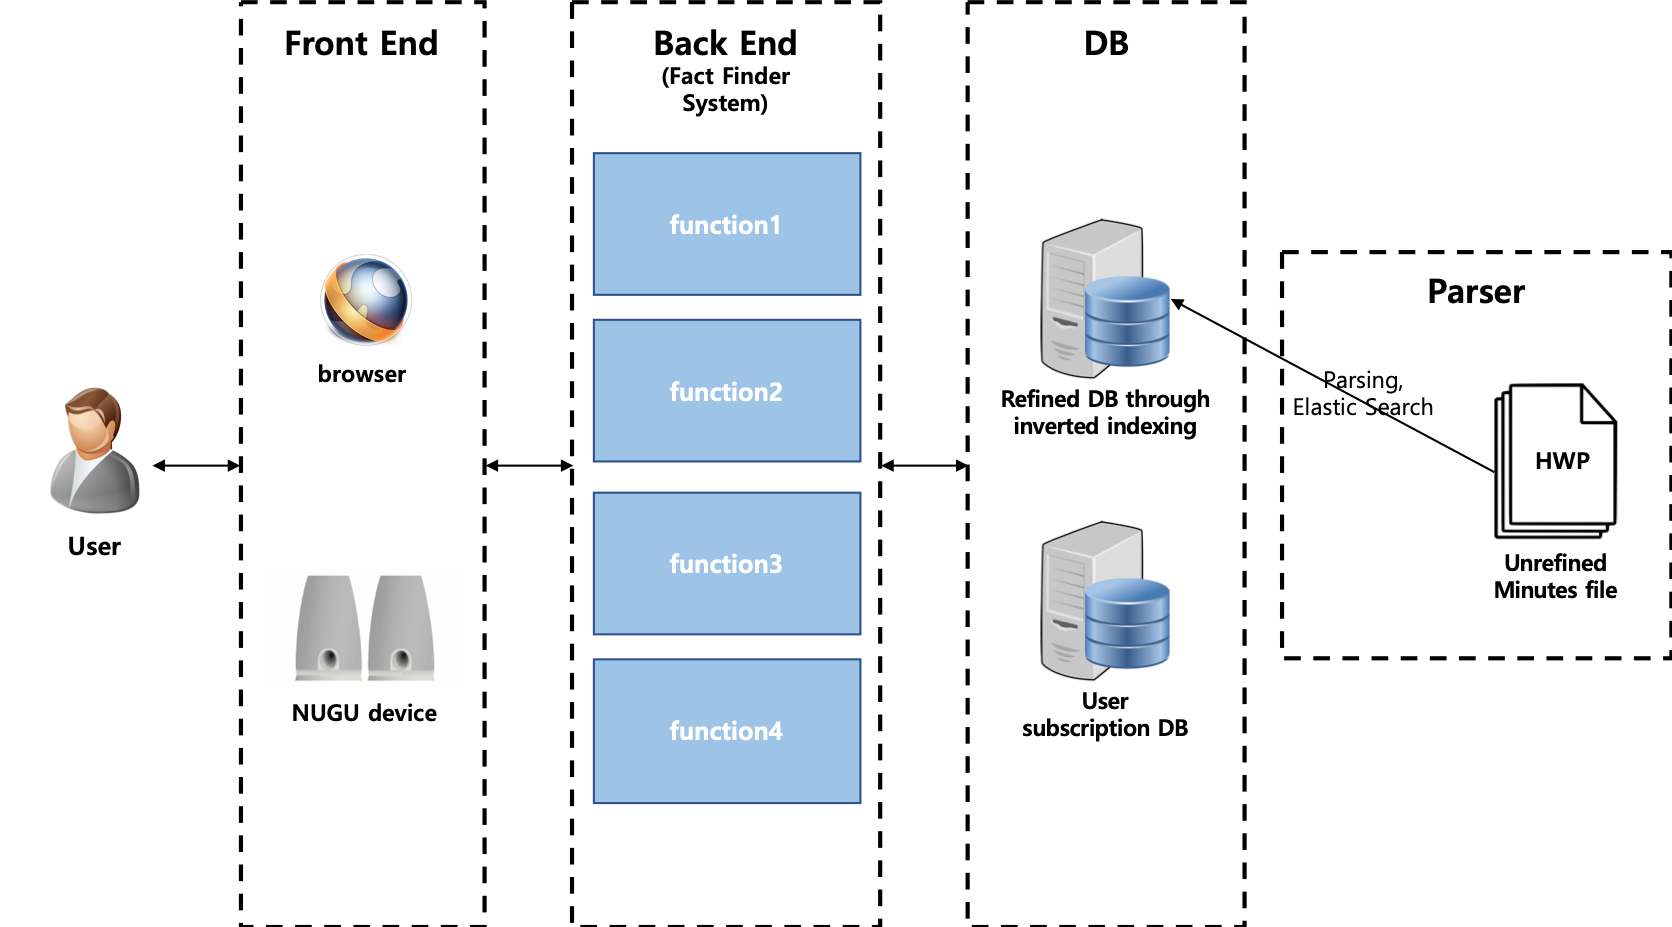
\includegraphics[width=100mm,scale=0.5]{fig/6_1.png}}
	\caption{Overall system architecture}
	\label{fig}
	\end{figure}
\vspace{5000mm}

\begin{figure}[htbp]
	\centerline{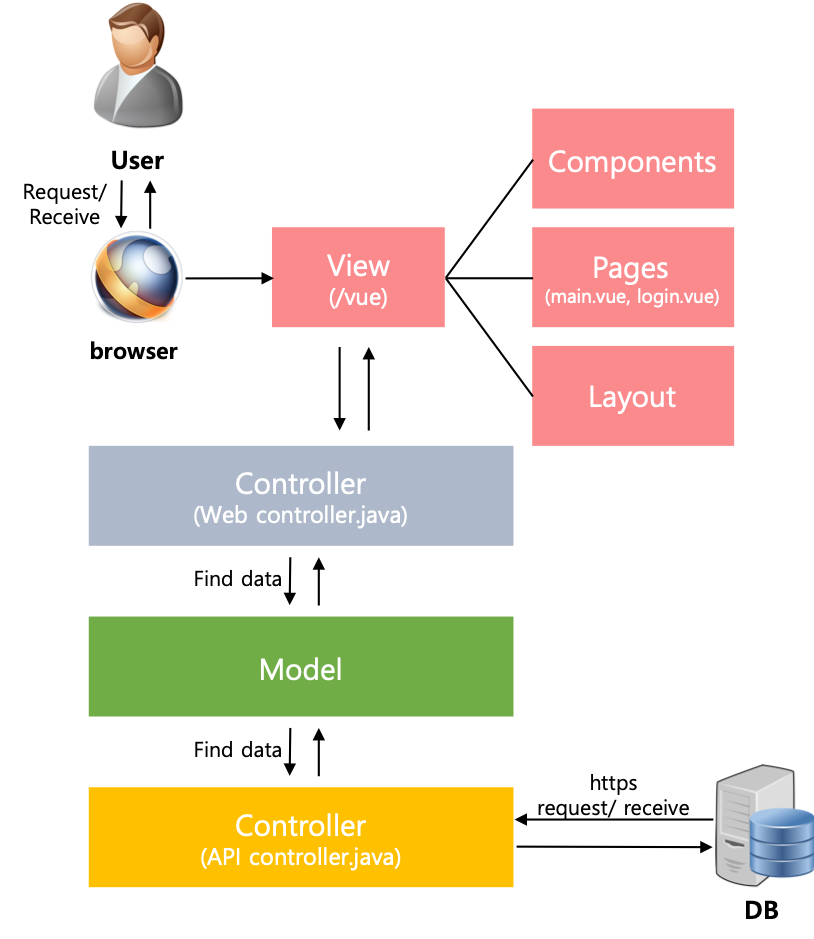
\includegraphics[width=70mm,scale=0.8]{fig/6_2.png}}
	\caption{MVC}
	\label{fig}
	\end{figure}
\subsection{Directory organization}
\vspace{500mm}

  \begin{table}[htbp]
  \renewcommand{\arraystretch}{1.5}
\caption{Directory organization}
\begin{center}
\begin{tabular}{|p{2.5cm}|p{4.3cm}|p{1cm}|}
\hline
\textbf{Directory} & \textbf{File names } &\textbf{Module name} \\
\hline
\multirow{7}{*}{/data\_preprocessor\_unit}& \_\_init\_\_.py&Parser \\
& congress\_member\_list\_preprocessor.py&\\
& data\_uploader.py &\\
& file\_manager.py &\\
& hwp\_to\_text.py & \\
& requirements.py & \\
&text\_preprocessor.py& \\

\hline
\multirow{3}{*}{frontend/} & nuxt.config.js&Web frontend \\
& package-lock.json & \\
& package.json & \\

\hline
\multirow{4}{*}{frontend/components}& CongressMemberList.vue& Web frontend\\
& Header.vue&\\
& MeetingLogList.vue & \\
& OrdinalList.vue & \\

\hline
\multirow{2}{*}{frontend/layouts} & HeaderLayout.vue& Web frontend\\
& deafault.vue &\\

\hline
\multirow{8}{*}{frontend/pages} & CongressMemberListView.vue & Web frontend\\
& LoginView & \\
& PlenarySessionBySeriesView.vue & \\
& ProfileView.vue & \\
& SignUpView.vue & \\
& SubscriberListView.vue & \\
& UnifiedSearchView.vue & \\
& index.vue & \\
\hline
\multirow{2}{*}{frontend/plugins} & bootstrap.js & Web frontend\\
& fontawesome.js & \\
\hline
\multirow{2}{*}{frontend/store} & index.js & Web frontend \\
& session.js & \\
\hline
\end{tabular}
\label{tab1}
\end{center}
\end{table}

\subsection{Module 1: Web Frontend}

\begin{figure}[htbp]
	\centerline{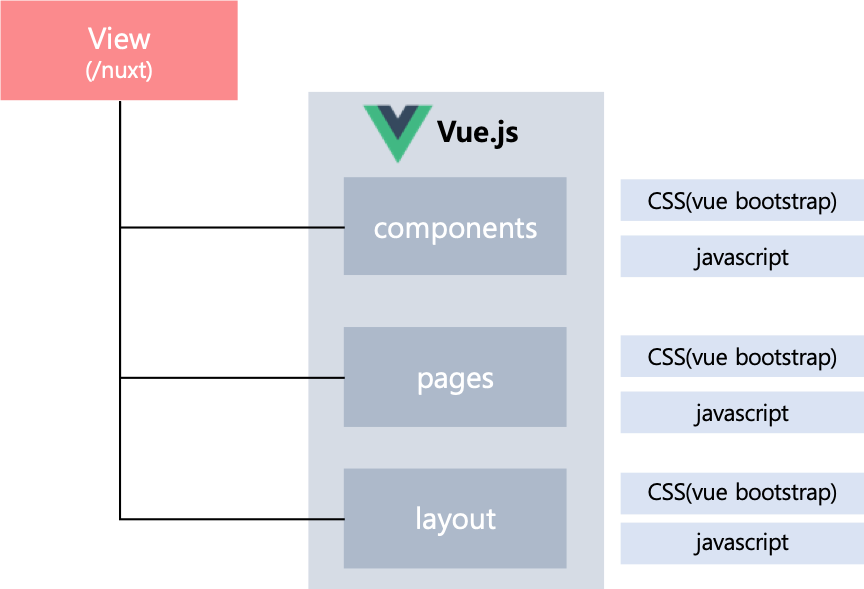
\includegraphics[width=90mm,scale=0.5]{fig/6_4.png}}
	\caption{Module 1: Web Frontend}
	\label{fig}
	\end{figure}
\vspace{500mm}

\begin{figure}[htbp]
	\centerline{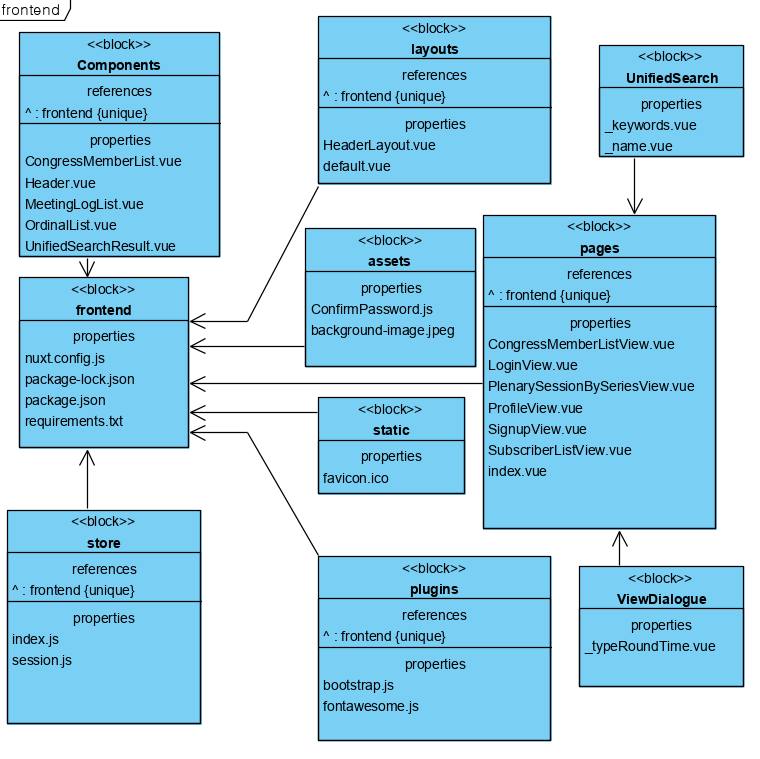
\includegraphics[width=90mm,scale=0.5]{fig/6_5.png}}
	\caption{Web Directory organization}
	\label{fig}
	\end{figure}
	
\begin{enumerate} 
  \item \textit{Purpose: } The purpose of the Web front-end is to provide our visualized functions to users. Users can request their needs through Web front-end and can deliver their request to the back-end without knowing inner service structure. Our web front-end’s roles in our projects is like below.
First, Users can’t memorize each of backend and Elasticsearch commands. So the web front-end must provide easy structure of service to receive the request of user’s needed information through single click..
Second, the users are provided a lot of information in once. So our web front-end should be constructed with a framework that provide information in fast and easy to use.
Third, The structure of the web front should be developed quickly. Our current projects need to construct four main functions, furthermore, the NUGU speaker functions, so our project team don’t have sufficient time to implement a lot of functions. \\
  \item \textit{Functionality: } 	
 \begin{enumerate}
	\item \textit {Vue.js: }  
	 \begin{enumerate}
	\item \textit {Virtual DOM function:} DOM(Document Object Model) is a interface of the web page. It provides API that many programs read and operate web page’s contents, structures, and style. Although, If the web service provide more and more user interfaces an interactions, managing and organizing that much DOM elements is going to be more harder. It is not impossible to setting a rule of fine conventions, but, it is still cumbersome. The Vue.js provides DOM management and minimize states update managements when developing web service. Thereby the developer can concentrate on implementing web functions and user interfaces.
	\item \textit {SPA(Single Page Application) function:} Vue.js provides SPA. A single-page application (SPA) is a web application or web site that interacts with the user by dynamically rewriting the current page rather than loading entire new pages from a server. This approach avoids interruption of the user experience between successive pages, making the application behave more like a desktop application. In a SPA, either all necessary code – HTML, JavaScript, and CSS – is retrieved with a single page load, or the appropriate resources are dynamically loaded and added to the page as necessary, usually in response to user actions. The page does not reload at any point in the process, nor does control transfer to another page, although the location hash or the HTML5 History API can be used to provide the perception and navigability of separate logical pages in the application. Interaction with the single-page application often involves dynamic communication with the web server behind the scenes.
	\item \textit {Reactive data processing function:} Vue.js provides Reactive data processing function. Along with the data is updated, referencing virtual DOM elements are also should be updated. We don’t need to find corresponding DOM element and change texts, because Vue.js does this function automatically.
	\item \textit {Reusing codes through components.:} Components means the block that can be combined and can struct screen. When using components, the developers can implement the View by constructing the screen fast in consistent patterns. it helps to understand the codes and reuse of the codes easily. By the components, The Javascript and HTML/CSS are divided and managed separately. So the maintenance become easy and it each codes can be reused. The scale of components can be configured by the developer. Therefore, the components is important in Vue.js Framework and the way of creation of components determines Vue.js’s developing speed, readability and effectiveness of codes.\\
	  \end{enumerate}
	  
	\item \textit {Nuxt.js: }Nuxt.js is a framework that can help to make Vue.js applications easily and improve productivity.\
		 \begin{enumerate}
		\item \textit {The UI rendering makes abstractions of client/server distribution. Just by installing Nuxt.js, it scaffolds(makes the project structured) the projects, so the developer can relieve the worry about the project structure.}  
	\item \textit { Nuxt.js predefines the configuration to help the developer to implement every structure that needed by the server-side rendered Vue.js application.}\\
	  \end{enumerate}

  \end{enumerate}
  \item \textit{Location of Source Code: } software engineering/frontend/\\

  \item \textit{Class component: } 
    \begin{enumerate}
	\item \textit {Vuex: }  Vuex is a manager of the virtual DOM. It observes the change of individual elements and updates them.\\
	\item \textit {Vue CLI:}Vue CLI(Vue Command Line Interface) makes and set up the projects automatically. It gathers Webpack, the package that gathers functions used by web developing, end configurate fundamental settings through several clicks. It is similar to NPM, the Node Package Manager, because the Vue CLI is activated through NPM.\\
	\item \textit {Vue Router:} Vue Router helps Vuex to manage Virtual DOM easily. In other words, It routes the way of what elements to be taken care of by the Vuex. By setting up individual elements on Vuex and drag it into the Vue router, the developer can reuse that elements to other functions.\\
	\end{enumerate}
  \item \textit{Where it is taken from: } Vue.js is developed by Evan You, who used AngularJS in various projects in google. The source code of Vue.js in in “https://github.com/vuejs/vue” and we used this package into our projects for our purpose.\\
  \item \textit{How and Why we use it: } We will fully use the productivity of Vue.js technique. We uses Vue.js technique to achieve the purpose of web front-end. Our current project have to implement four core functions and NUGU speaker function. Our team decided to use Vue.js javascript framework because of its lower entry barrier, flexibility, high performance, and easier maintenance and testing environment. The Vue.js officially supports build system, routing, status management that needed to used in real service so we can develop our environment very fast. Also we will use Nuxt.js to enhance our developing productivity because it helps to abstract server and distribute our service.\\
  \end{enumerate}


\subsection{Module 1.b: NUGU speaker frontend}
\begin{figure}[htbp]
	\centerline{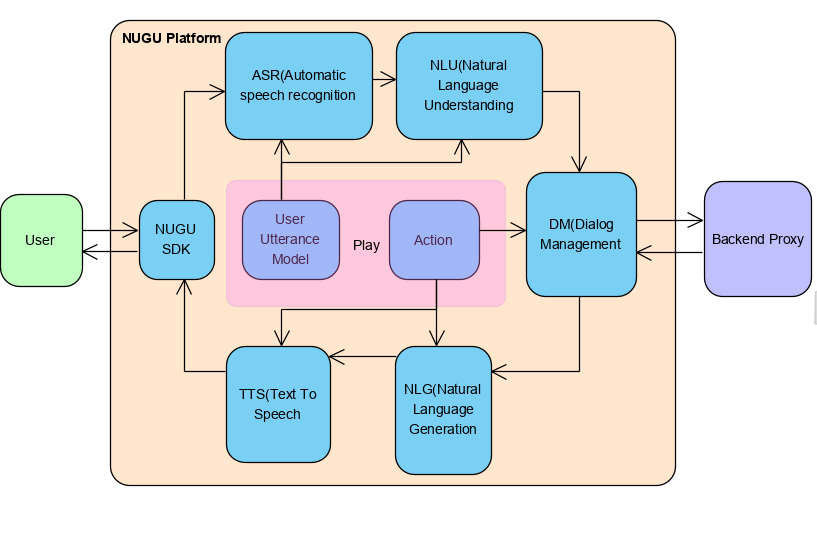
\includegraphics[width=90mm,scale=0.5]{fig/6_7.png}}
	\caption{Web Directory organization}
	\label{fig}
	\end{figure}
	
\vspace{30mm}
\begin{enumerate} 
  \item \textit{Purpose: } The biggest difference between web front-end and NUGU speaker front-end is that the web front-end communicates with user as visualized, and the NUGU speaker front-end communicates with user as sound. It is the first core roles to communicate with NUGU AI speaker. Second, it must built on stable by training the system through NUGU play builder to reduces frequency of exception rate. Third, it has to communicate with our back-end without errors by setting up RESTful each action.\\
  \item \textit{Functionality: } 	
 \begin{enumerate}
	\item \textit {Doesn’t need coding skill: }  NUGU play builder that made by SKT for developers makes the developer to implement what he wants without programming skill. The GUI interface doesn’t require coding phase, except for if the developer wants to get information from his system.\	  
	\item \textit {Automatic voice recognition: }The internal built-in technique such as Automatic Speech Recognition, Natural Language Understanding, Dialog Management, Natural Language Generation, Test To Speech automatically recognize user utterances and makes appropriate response to the user.\
	\item \textit {Communicate with backend proxy: }Only with the NUGU play builder, the developer can’t make own system that communicates with other server. The developer should make own RESTful server and controller to deliver values to the NUGU play builder, eventually, to user.\\
  \end{enumerate}
  
  \item \textit{Location of Source Code: } https://builder.NUGU.co.kr/\\

  \item \textit{Class component: } 
  	 \begin{enumerate}
	\item \textit {Intents: }  It means prediction of user utterance after NUGU play made. It should be defined beforehand of user utterance. NUGU play ties up user utterances that intend to activate specific function.\
	 \begin{enumerate}
	\item \textit {PFF subscribe: } User can subscribe specific politician through this intent. The politician name defined in Entity types should be tied up with this intent to implement this intent.
	\item \textit {PFF agendalist:} User can be returned specific agenda which specific politician was participated. The politician name defined in Entity types should be tied up with this intent to implement this intent.
	\item \textit {PFF politicianlist:} User can be returned politician list that user was subscribed. The politician list should be saved in our database to return to the user.
	\item \textit {PFF recent discussion:} User can be returned specific discussion which specific politician was participated. The politician name defined in Entity types should be tied up with this intent to implement this intent.\\
	  \end{enumerate}

	\item \textit {Entity types: }  The Entity type should be predefined to match up intents. If it is not predefined and tied up with intents, the NUGU speaker can’t understand what the user want to mean.\
	 \begin{enumerate}
	\item \textit {POLITICIAN NAME: } Politician name was predefined to be tied up with intents. All of the politicians should be predefined manually in this entity type.
	  \end{enumerate}
	  
	  	\item \textit {Actions: }  Our custom actions should be predefined to match up with intents. In this, predefined intents become the trigger to get return information. The parameters get from the our backend controller will be returned to the user.\
	 \begin{enumerate}
	\item \textit {subscribeAnswer: } It is tied up with intent, PFF subscribeAnswer. User can subscribe specific politician through this intent. The politician name defined in Entity types should be tied up with this intent to implement this intent.
	\item \textit {agendaAnswer: } It is tied up with intent, PFF agendalist. User can be returned specific agenda which specific politician was participated. The politician name defined in Entity types should be tied up with this intent to implement this intent.
	\item \textit {politicianlistAnswer:} It is tied up with intent, PFF politicianlist. User can be returned politician list that user was subscribed. The politician list should be saved in our database to return to the user.
	\item \textit {recentdiscussionAnswer: } It is tied up with intent, PFF recent discussion. User can be returned specific discussion which specific politician was participated. The politician name defined in Entity types should be tied up with this intent to implement this intent.
	  \end{enumerate}
	  	  \end{enumerate}
		  
	    \item \textit{Where it is taken from: } It is from NUGU developer site, “https://developers.NUGU.co.kr/” and its document is from “https://developers-doc.NUGU.co.kr/”.\\
  \item \textit{How and Why we use it: } By predefining all of intents, entities and actions we can submit this Play(A whole front-end service) to the client(SKT), and if they approve this system, finally user can use our voice front-end service.
We used NUGU play builder because through this we can easily make prototype of AI intercommunicating speaker platform. Also, the client, SKT, demanded to make a complete system that have a potential of commercializing.\\
  \end{enumerate}
  
  
  \subsection{Module 2: backend}
\begin{figure}[htbp]
	\centerline{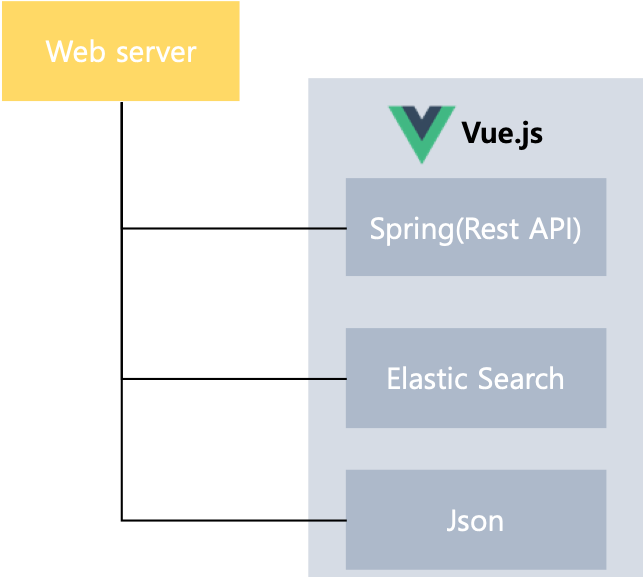
\includegraphics[width=90mm,scale=0.5]{fig/6_6.png}}
	\caption{Module 1: Web Frontend}
	\label{fig}
	\end{figure}
	
\vspace{30mm}
\begin{enumerate} 
  \item \textit{Purpose: } The purpose of the back-end is to process of the user request that is from the front-end. If the user requests something from our front-end service, the back-end receives that request and delivers the message to our Database and receive the response data, and filters information that the front-end needs. Originally the database can be included in the back-end, but we made our database through the Elasticsearch separately, and we will discuss it as a separate module.
Our back-end purpose is like below. First, It should perform the functions that the front-end requests. Second, It should gives and takes values from Elasticsearch database to perform the functions that the front-end requests.
For that purposes, We used Spring framework, that is based on Java language. The Elasticsearch provide response based on json format, we developed API controller that uses HTTPS, RESTful protocol to communicate with our database. Also, we developed Web controller to process requests from our web service, and NUGU controller that process requests from NUGU speaker. Through our back-end module, we can provide refined requests data to users.\\
  \item \textit{Functionality: } 	
  	 \begin{enumerate}

	\item \textit {Spring: }   The Spring Framework is an open source application framework and inversion of control container for the Java platform. The framework's core features can be used by any Java application, but there are extensions for building web applications on top of the Java EE platform.
	 \begin{enumerate}
	\item \textit {MVC pattern:} A business logic, MVC(Model View Controller) is a design pattern that places Controller between Model and View to separates them. Spring uses Front Controller pattern to implement MVC pattern as other web MVC framework, and it is laid out with servlet that provide several functions of this framework. The DiapatcherServlet takes role of Front Controller in the Spring, furthermore, it is integrated with IoC container to use all of other functions of Spring, and supervise web request life cycle. So, The Spring DispatcherServlet is the Spring MVC’s core elements. Specifically in our project, the Vue.js takes the role of View, and the Spring Controller function as RESTful to change preexistence Model domain roles to HTTP json protocol.
	\item \textit {Batch framework:} Spring provides batch framework that supports batch processing. The batch processing is used for processing a lot of data or executed in specific time. Basically the Spring batch framework is operated on Quartz.
	  \end{enumerate}
	  
	\item \textit {Tomcat: }The tomcat is called as a Web or servlet container to build dynamic web. The dynamic elements as JSP, ASP, PHP are delivered to the Tomcat except for static data like CSS.\
  	  \end{enumerate}

  \item \textit{Location of Source Code: } https://builder.NUGU.co.kr/\\

  \item \textit{Class component: } 
  	 \begin{enumerate}
	\item \textit {Web controller: }  \
	 \begin{enumerate}
	\item \textit {Method1: }  If user sends information of specific meeting’s id number, it returns specific meeting and number of meeting to View
	\item \textit {Method2: } If user sends information of meeting or meeting number, Return specific agenda and discussion to the front controller
	\item \textit {Method3: } If user sends information of specific meeting’s id number, it returns politician’s name and his party to the front controller
	\item \textit { Log-in:} If user sends right information of id and password, it returns successful status message to the View
	\item \textit { Subscribe:} If user send message that he wants to subscribe specific politician, It make the politician subscribed
	\\
	 \end{enumerate}

	\item \textit {NUGU controller: }  \

	 \begin{enumerate}
	\item \textit {Method1: }   If the user send information of politician’s name, it returns information of meeting and number of meeting that politician’s participated.
	\item \textit {Method2: } If the user send information of politician’s name, it returns information of agenda that politician’s participated.
	\item \textit {Method3: } If the user requests subscribed list, it returns politician subscribed list.
	\\
	  \end{enumerate}
	  
	  
	 \item \textit {API controller: }  \

	 \begin{enumerate}
	\item \textit {Method1: }If the front controller send information of specific meeting’s id number, it returns specific meeting and number of meeting to the front controller	
	\item \textit {Method2: } If the front controller send information of meeting or meeting number, Return specific agenda and discussion to the front controller
	\item \textit {Method3: }  If the front controller send information of specific meeting’s id number, it returns politician’s name and his party to the front controller
	\item \textit {Method4: }  If the front controller send information of politician’s name, it returns specific meeting information and discussion to the front controller
	\\
	  \end{enumerate}
	  \end{enumerate}	  
		  
	    \item \textit{Where it is taken from: } The Spring is the open source application framework for Java platform. The source code of Spring of Spring is in “https://github.com/spring-projects/spring-framework” and we used this package into our project for our purpose. We build API controller, NUGU controller, Web controller through this package and add pages to refine our functions.\\
  \item \textit{How and Why we use it: } We will use Spring framework and we will build Spring MVC pattern for our purpose. In our project, Vue.js is used for View part. Also, the database will be built on Elasticsearch software. The elasticsearch give and takes information on json format. So our back-end controller will be built like RESTful to change preexistence model domain roles to HTTP json protocol to communicate with our database. Furthermore, the Web controller and NUGU controller is built on Restful because the front-ends are also communicate with RESTfully, and it gives universality and unity to overall structure. The controllers in our Spring framework will provide responses with refined data on user requests.\\
  \end{enumerate}

  
  \subsection{Module 3: Database(Elasticsearch)}
\begin{figure}[htbp]
	\centerline{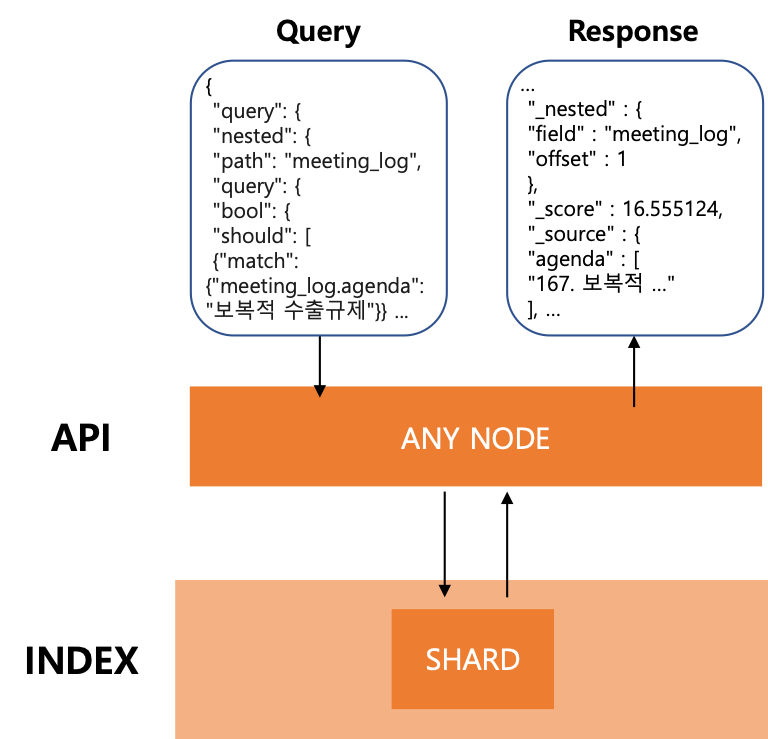
\includegraphics[width=90mm,scale=0.5]{fig/6_8.png}}
	\caption{Module 1: Web Frontend}
	\label{fig}
	\end{figure}
	
\vspace{30mm}
\begin{enumerate} 
  \item \textit{Purpose: } One of our main function, Searching real speech of the politician should be developed on exquisite searching algorithm. The Elasticsearch supports very delicate searching function through inverted indexing. Also, the speed of the service decides the steady use of our service. That is, using this database determines our service’s life or death. So our team decided to use this system.\\
  \item \textit{Functionality: } 	
  	 \begin{enumerate}

	\item \textit {No-schema storage that based on json format: }   Although the elasticsearch is a search engine, but it can be used as NoSQL. Elasticsearch uses data model as a json, so sending requests and receiving responses are conducted on json document, and saving source to json format. Even if the developer doesn’t predefined schema, this engine indexes the json format data automatically. The number or date types are also mapped automatically.\
	  
	\item \textit {Multi-tenancy: }Elasticsearch support multi-tenancy. By storing several indexes in only one elasticsearch server, the controller can receive search results by sending only one query the data in several indexes. For example, even if the data is separated by dates, the one query can get results by adjusting the searching range.\
	
	\item \textit {Expandability and flexibility: }Elasticsearch’s expandability and flexibility are very outstanding. The developer can expand functions through plug-in. The developer can change transport protocol by using Thrift or Jetty plugin. Also, the developer can use elasticsearch monitoring function by installing BigDesk or Head plugin. We can be provided far more accurate, visualized statistics through extendable plug in.\
		
	\item \textit {Distributed storage: }The elasticsearch is distributed storage. The data can be distributed by keys, several shards are constructed. Indexes are constituted by each shards. Each shards has more than 0 replicas. Elasticsearch supports clustering, and when the cluster activated, one of the nodes is elected as a master node to manage mata-data. If the master node goes down, another node in cluster becomes master node. Adding node is also very easy. The characteristic of distributed storage makes the database more fast and more safe.\
			
  	  \end{enumerate}

  \item \textit{Location of Source Code: } https://builder.NUGU.co.kr/\\

  \item \textit{Class component: } 
  	 \begin{enumerate}
	\item \textit {Request queryr: }  The request query’s format is formatted on json. The request json query have two field components. If the user enter some words in the search bar in our service, their words will filled in the URL parameter to send request query to our database.\
	 \begin{enumerate}
	\item \textit {path: }  path specifies where to find the result.\
	\item \textit {match: } match specifies what to search. The match keyword  is filled in both agenda and discussions, that will be separated from the results.\
	\\
	 \end{enumerate}
	 
	 
	\item \textit {Response message: }  The request message is also formatted on json. The response json message have several response data. These informations will become the result in the front end.
	 \begin{enumerate}
	\item \textit {index: }  It is similar to RDBMS’s table. specifically, It exhibits Nth Congress meeting of the Nth National Assembly.\
	\item \textit {id: } It exhibits the round number of Nth congress meeting.\
	\item \textit {field: } It’s like RDBMS’s column. field specify where to request the data.\
	\item \textit {offset: } It means what number of the utterances in agenda.\
	\item \textit {score: } IIt means that the similarity between searching keyword and the result data. By descending the order of score, user can get the most similar result.\
	\item \textit {agenda: }  It means the agenda of corresponding result.\
	\item \textit {discussion: }It means the whole utterances of politicians in the result.\
		\\
	 \end{enumerate}
	 
		 \end{enumerate}

		  
	    \item \textit{Where it is taken from: } This software is made by Elastic NV. Elastic NV is a company that was founded in 2012 in Amsterdam, the Netherlands, and was previously known as Elasticsearch. The source code of Elasticsearch can be viewed in “https://github.com/elastic/elasticsearch”.\\
	    
  \item \textit{How and Why we use it: } Automated system makes query that composed on json format to be delivered to the Database. The result of that query will appear The speed of searching is very fast if we use Elasticsearch. Based on Similarity measure system in the Elasticsearch produces more accurate result to user in effort.  The searching algorithm that implemented through inverted indexing makes our service far more faster. Besides, even though its functionality, it is open source so it is free to use if not for commercial use.\\
  \end{enumerate}
  
  
  
  
  
  
    \subsection{Module 4: Parser}
\begin{figure}[htbp]
	\centerline{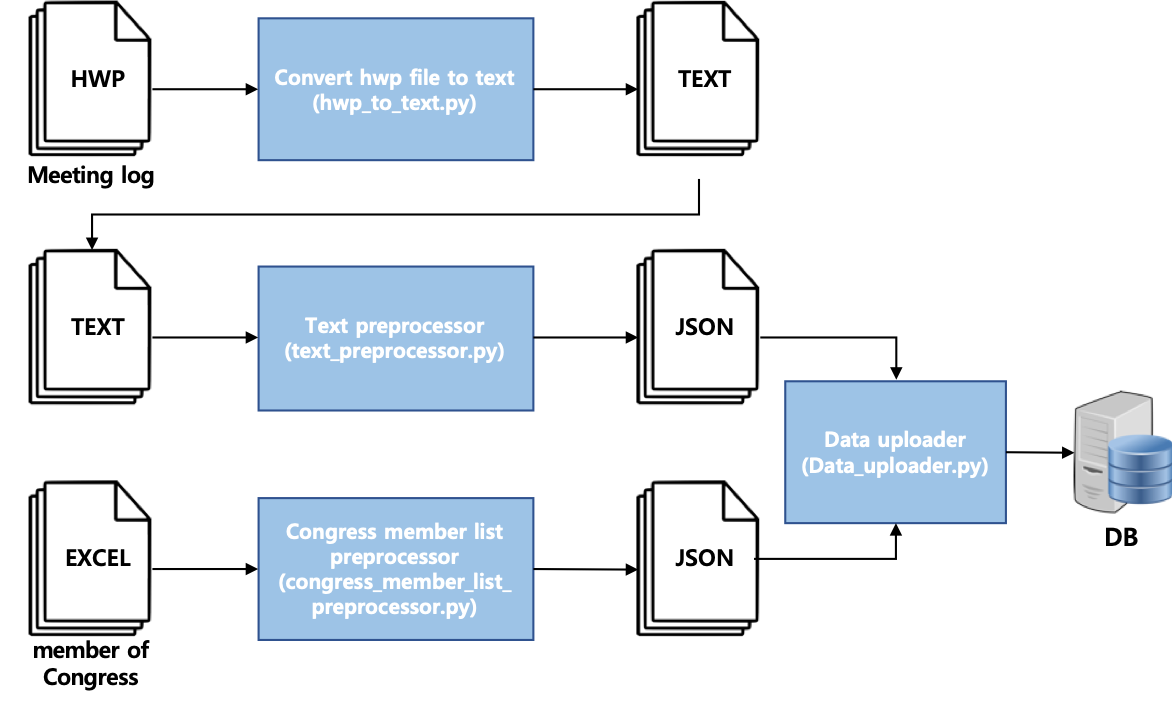
\includegraphics[width=90mm,scale=0.5]{fig/6_9.png}}
	\caption{Module 1: Web Frontend}
	\label{fig}
	\end{figure}
	
\begin{figure}[htbp]
	\centerline{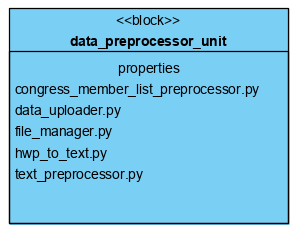
\includegraphics[width=90mm,scale=0.5]{fig/6_10.png}}
	\caption{Module 1: Web Frontend}
	\label{fig}
	\end{figure}
	
\vspace{30mm}
\begin{enumerate} 
  \item \textit{Purpose: } Our service’s purpose is to  provide Assembly minutes and its data to the users. The core data that we want to provide is uploaded on the assembly minutes site, but its files location and forms and are too complicated to see or find. So our team decided to refine these files to save our database. If this module doesn’t exist, The next further modules won’t be existed because of unorganized original formats.\\
  
  \item \textit{Functionality: } This module performs as a preprocessor of raw data. The raw data are formed with hwp file or pdf file. The chosen hwp file will be converted into the text, and finally with json format that can be uploaded to Database as well-organized.\

  \item \textit{Location of Source Code: } /data preprocessor unit/\\

  \item \textit{Class component: } 
  	 \begin{enumerate}
	\item \textit {Convert hwp file to text: }  This script convert hwp file that are downloaded from assembly minutes files to texts that should be refined after through text preprocessor. The hwp file can’t be uploaded to the Elasticsearch Database. The text file name is refactored by this file to the English name for afterward. What file that should be converted is managed by file manager.py\

	\item \textit {Text preprocessor: }  The text components converted by hwp to text.py will be parsed through this file. The contents of text file is so dizzy and didn’t organized. The contents will be parsed by  separators. The text file will be parsed by four components, “round plenary session, type, id, dialogue” on json format.\
	
	\item \textit {Congress member list preprocessor: }  The congress member list that can be downloaded from National Election Commision made of excel form will be converted through this preprocessor. the list of congress member will be organized with json format.\
	
	\item \textit {Data uploader: }  The json datas refined from above are finally saved to the Elasticsearch, our database.\
	\item \textit {File manager: }  The file manager decides what file to be converted to another format. it checks argv and manages the file to be read.\
	 
		 \end{enumerate}

		  
	    \item \textit{Where it is taken from: } Because of its unique characteristic of our algorithm, fit codes for our parsing system not much distributed from internet. So we had to fetch a few open source packages only like pyhwp, pathlib, dataclasses, multiprocessing, json, subprocess, re, openpyxl, elasticsearch.\\
	    
  \item \textit{How and Why we use it: } In first step, the hwp files are downloaded mannually by hands.This step will be converted further to be upgraded by crawlling data. Then, Operate hwp to text function should be processed to convert hwp format to text format, and text preprocessor converts text format to json format. Along with this steps, the congress member list preprocessor function also be operated to convert politician list excel files to json format. Finally, Operating the data upload function upoloads the json format data to Elasticsearch Database. The Elasticsearch database is updated based on NoSQL, so the data should be converted to json format to save to Database. So we should have to use this module to convert data to json format by exquisitely refining.\\
  \end{enumerate}
  
  
  
\end{document}
 
 

